\documentclass[pdflatex,compress,mathserif]{beamer}

%\usetheme[dark,framenumber,totalframenumber]{ElektroITK}
\usetheme[darktitle,framenumber,totalframenumber]{ElektroITK}

\usepackage[utf8]{inputenc}
\usepackage[T1]{fontenc}
\usepackage{lmodern}
\usepackage[english]{babel}
\usepackage{amsmath}
\usepackage{amsfonts}
\usepackage{amssymb}
\usepackage{graphicx}
\usepackage{multicol}
\usepackage{lipsum}
\usepackage{framed}
\usepackage{minted}

\definecolor{LightGray}{gray}{0.95}

\usefonttheme[onlymath]{serif}

\newcommand*{\Scale}[2][4]{\scalebox{#1}{$#2$}}%

\setbeamertemplate{caption}[numbered]

\title{Digital Signal Processing}
\subtitle{Finite Impulse Response}

\author{Mifta Nur Farid}

\begin{document}

\maketitle

\begin{frame}{FIR Filter Format}
    \begin{itemize}
        \item Difference equation:
        \begin{figure}
            \centering
            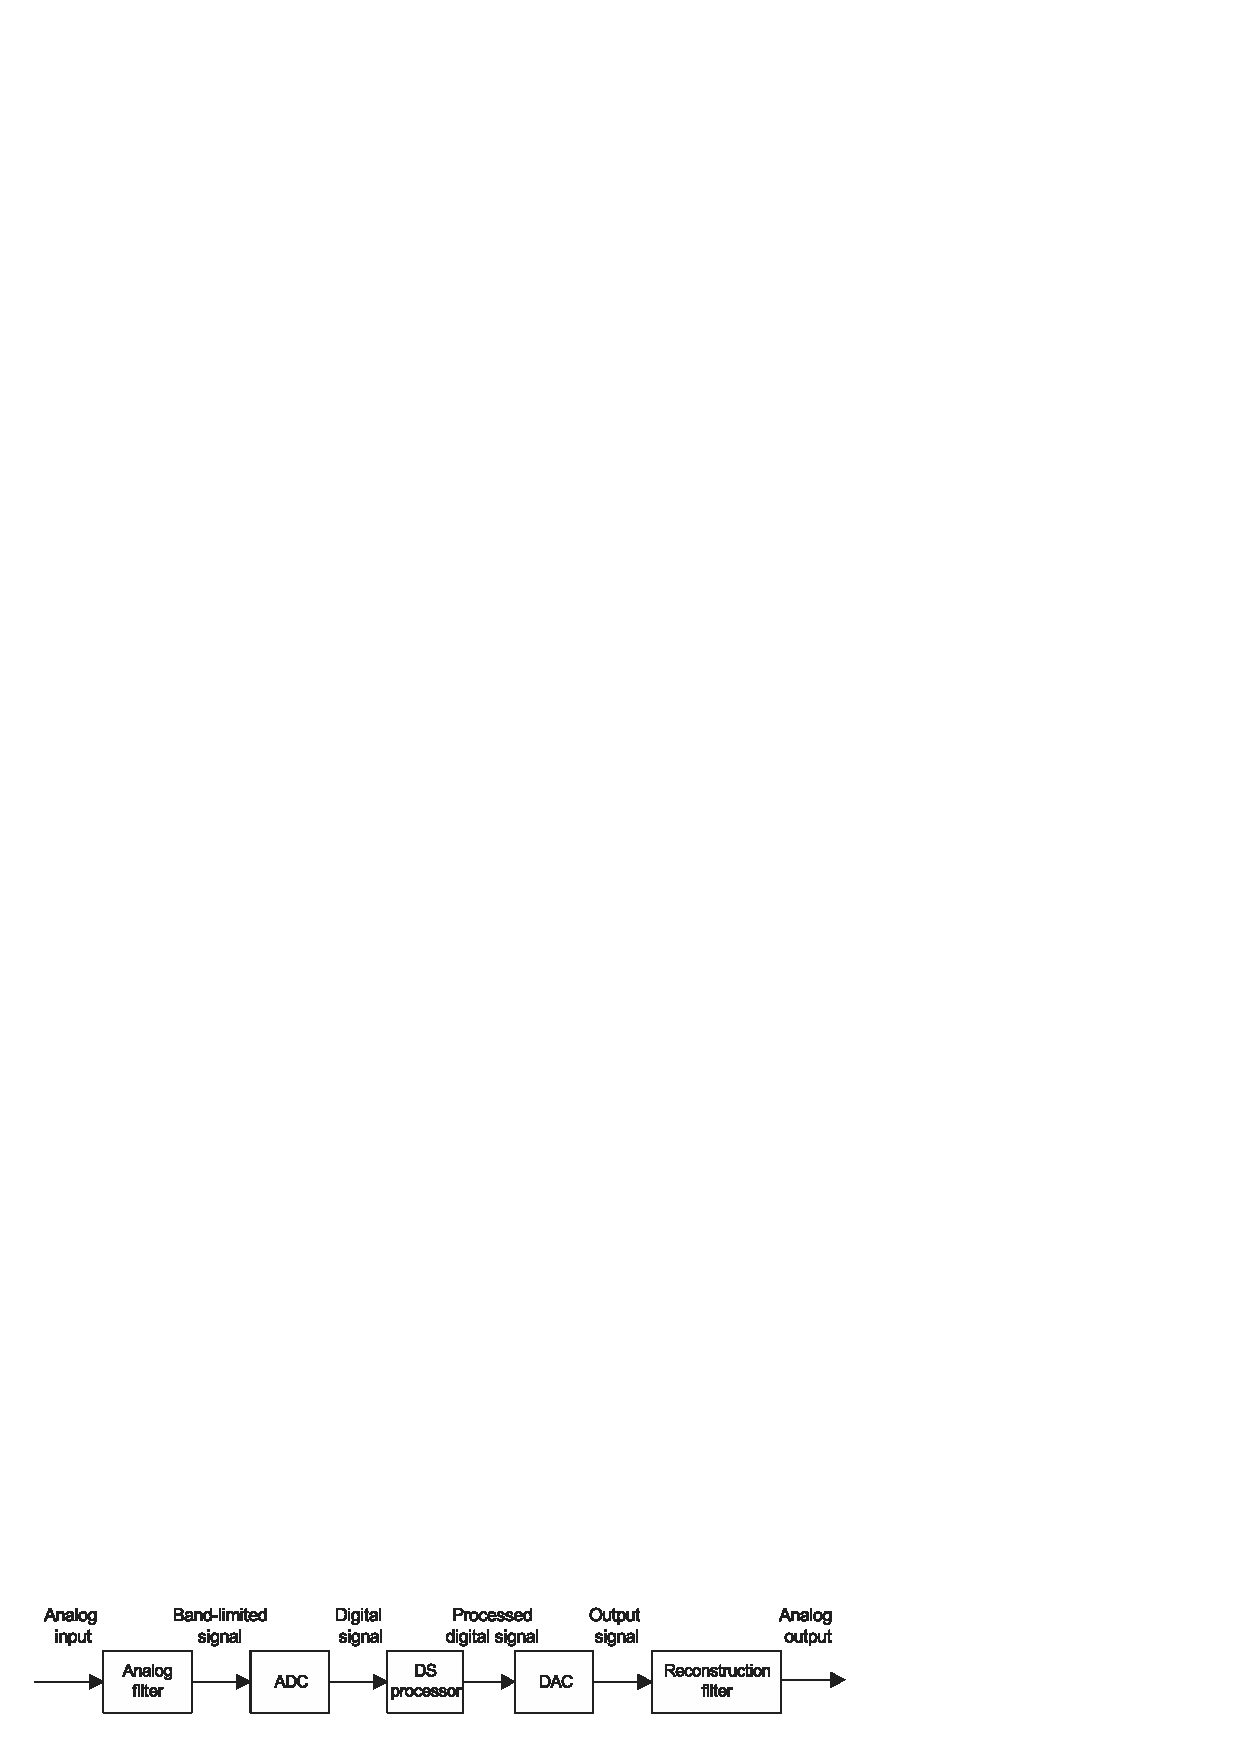
\includegraphics[width=0.8\linewidth]{./img/img01.png}
        \end{figure}
        $b_i$: FIR filter coefficients, $K+1$: FIR filter length
        \item in $z$-domain:
        \begin{figure}
            \centering
            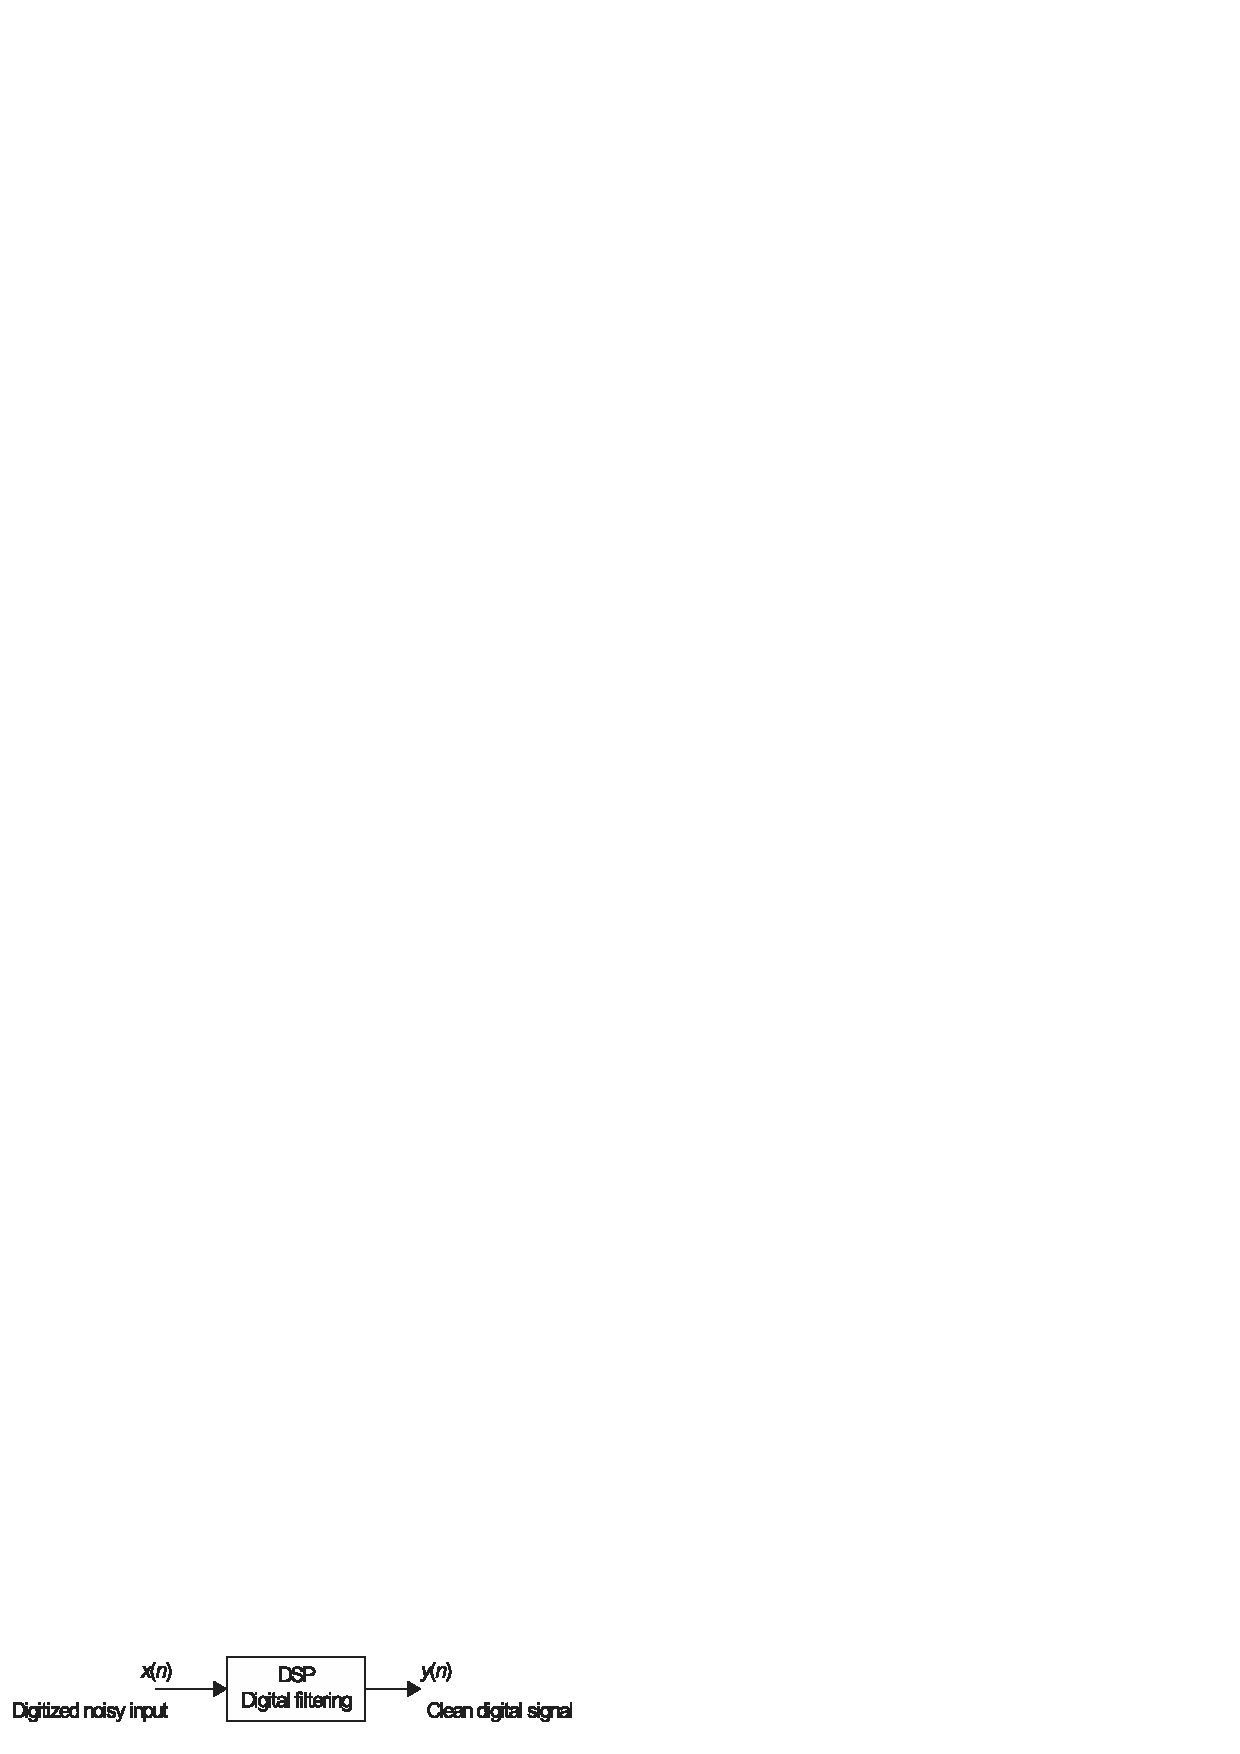
\includegraphics[width=0.6\linewidth]{./img/img02.png}
        \end{figure}
        \item transfer function:
        \begin{figure}
            \centering
            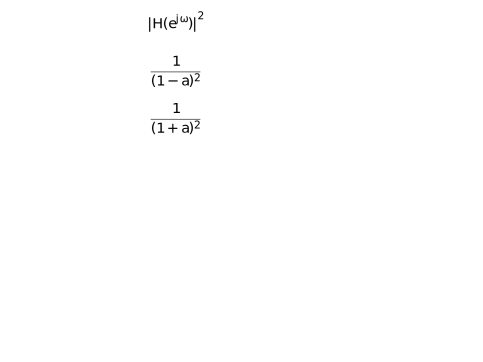
\includegraphics[width=0.5\linewidth]{./img/img03.png}
        \end{figure}
    \end{itemize}
\end{frame}

\begin{frame}{Example}
    \begin{itemize}
        \item Given the following FIR filter: $$ y(n) = 0.1 x(n) + 0.25 x(n-1) + 0.2 x(n-2) $$ Determine
        \begin{enumerate}[a.]
            \item the transfer function
            \item filter length
            \item nonzero coefficients
            \item impulse response
        \end{enumerate}
    \end{itemize}
\end{frame}

\begin{frame}{Solution}
    \begin{enumerate}[a.]
        \item the transfer function: applying $z$-transform $$ Y(z) = 0.1 X(z) + 0.25 X(z) z^{-1} + 0.2 X(z) z^{-2} $$ transfer function: $$ H(z) = \frac{Y(z)}{X(z)} = 0.1 + 0.25 z^{-1} + 0.2 z^{-2} $$
        \item filter length: $K + 1 = 2 + 1 = 3$
        \item nonzero coefficients: $b_0 = 0.1$, $b_1 = 0.25$, $b_2 = 0.2$
        \item impulse response: invers $z$-transform of the transfer function: $$h(n) = 0.1 \delta(n) + 0.25 \delta(n-1) + 0.2 \delta(n-2)$$
    \end{enumerate}
\end{frame}

\begin{frame}{FIR Filter Coefficients:\\Fourier Transform Design}
    \begin{itemize}
        \item Ideal Impulse Response $h(n)$ (Noncausal FIR coefficients)
        \begin{enumerate}[a.]
            \item Lowpass:
            \begin{figure}
                \centering
                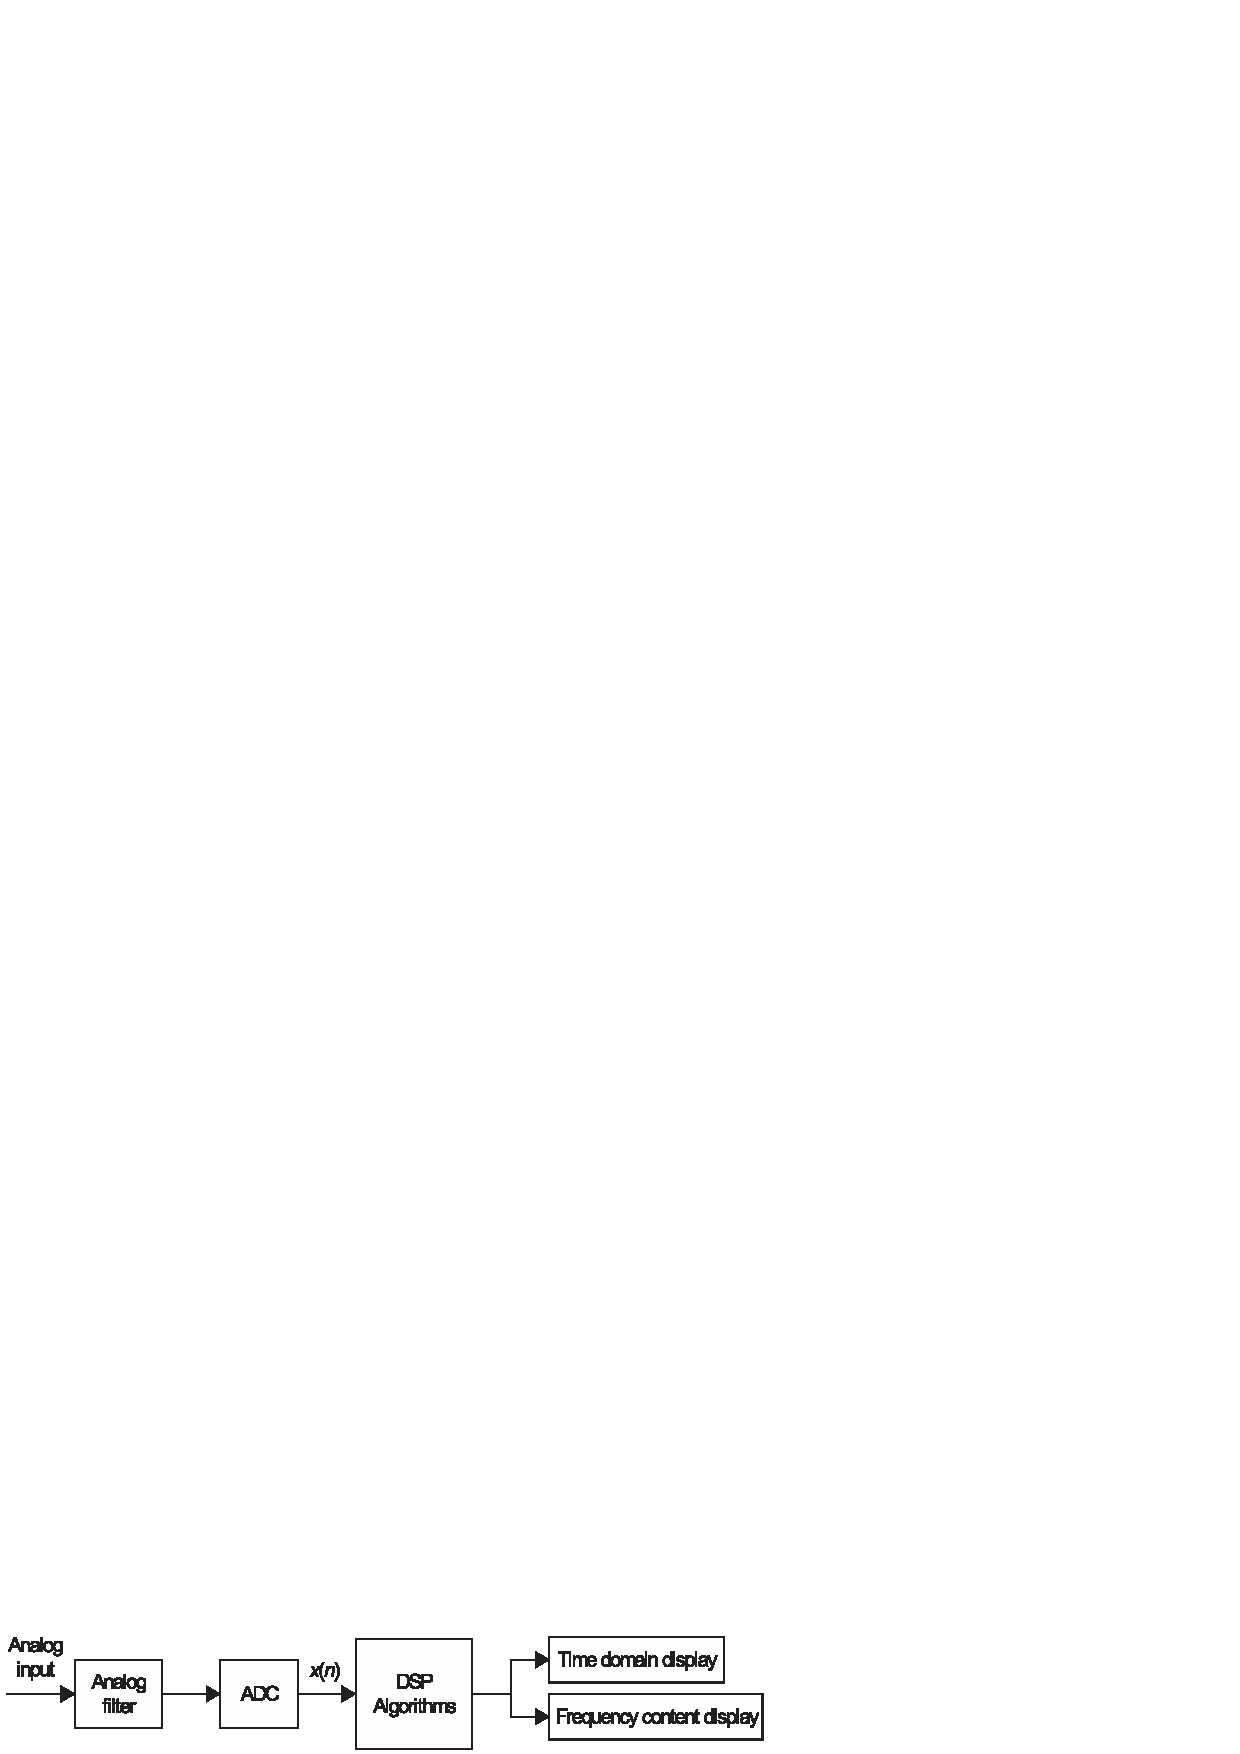
\includegraphics[width=0.7\linewidth]{./img/img04.png}
            \end{figure}
            \item Highpass:
            \begin{figure}
                \centering
                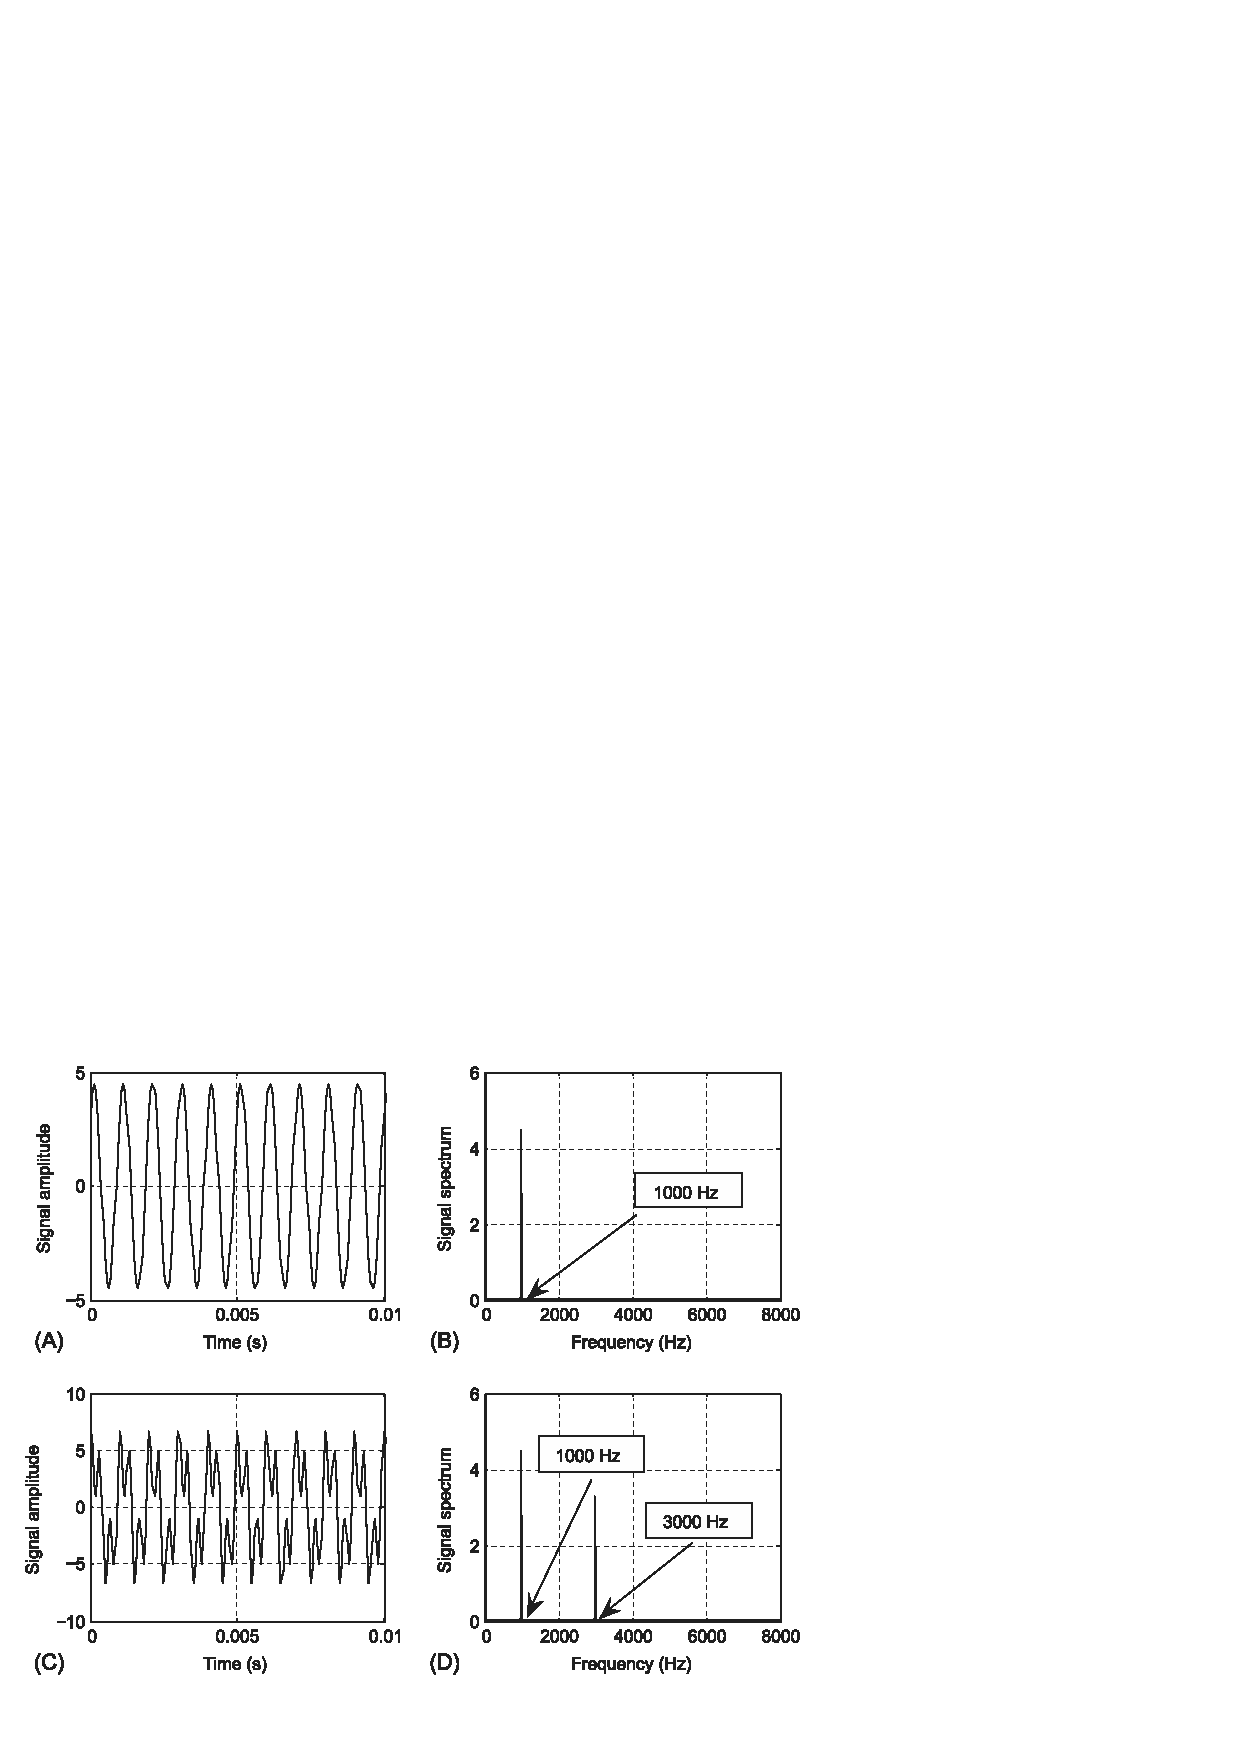
\includegraphics[width=0.7\linewidth]{./img/img05.png}
            \end{figure}
        \end{enumerate}
    \end{itemize}    
\end{frame}

\begin{frame}{FIR Filter Coefficients:\\Fourier Transform Design}
    \begin{itemize}
        \item Ideal Impulse Response $h(n)$ (Noncausal FIR coefficients)
        \begin{enumerate}[a.]
            \setcounter{enumi}{2}
            \item Bandpass:
            \begin{figure}
                \centering
                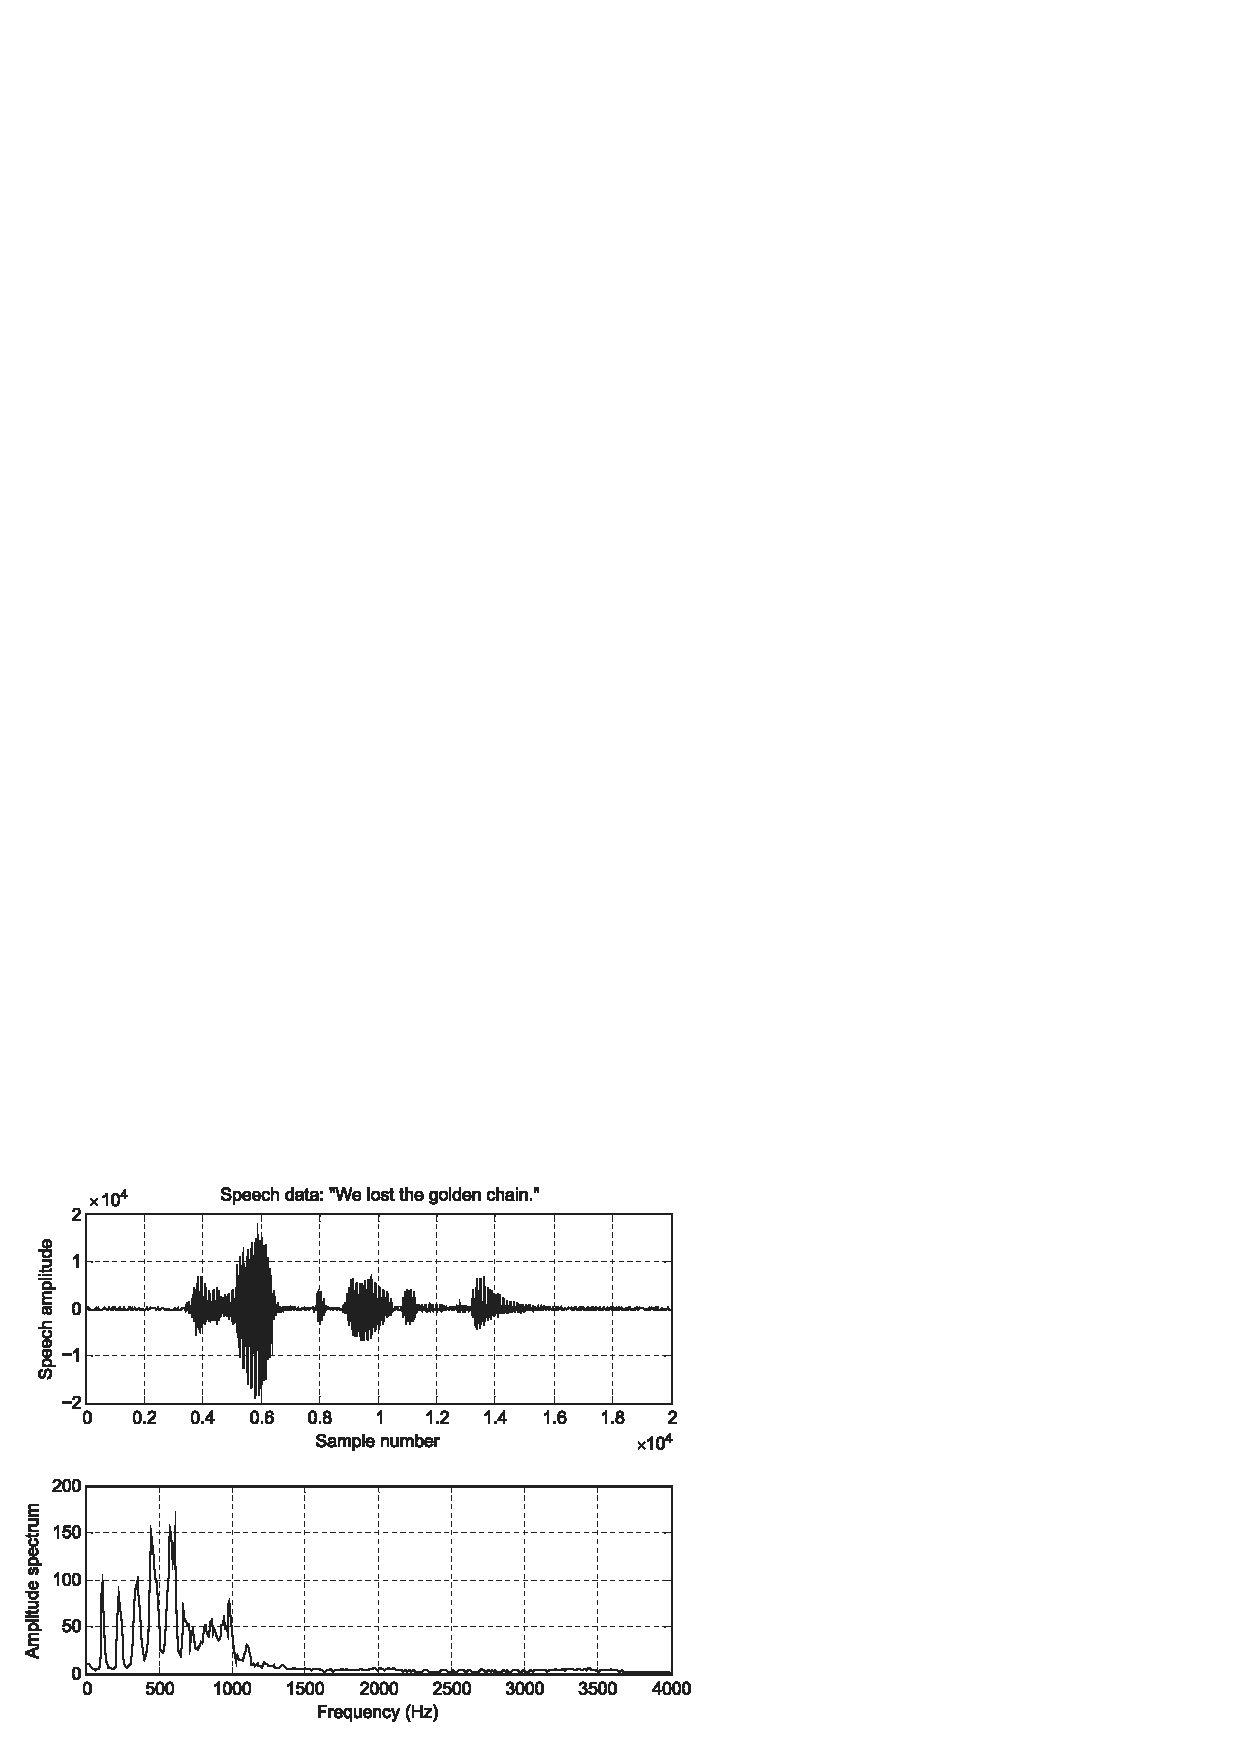
\includegraphics[width=0.8\linewidth]{./img/img06.png}
            \end{figure}
            \item Bandstop:
            \begin{figure}
                \centering
                \includegraphics[width=0.8\linewidth]{./img/img07.png}
            \end{figure}
        \end{enumerate}
    \end{itemize}    
\end{frame}

\begin{frame}{FIR Filter Coefficients:\\Fourier Transform Design}
    \begin{itemize}
        \item Causal FIR coefficients: shifting $h(n)$ to right by $M$ samples
        \item Transfer function:
        \begin{figure}
            \centering
            \includegraphics[width=0.6\linewidth]{./img/img08.png}
        \end{figure}
        where
        \begin{figure}
            \centering
            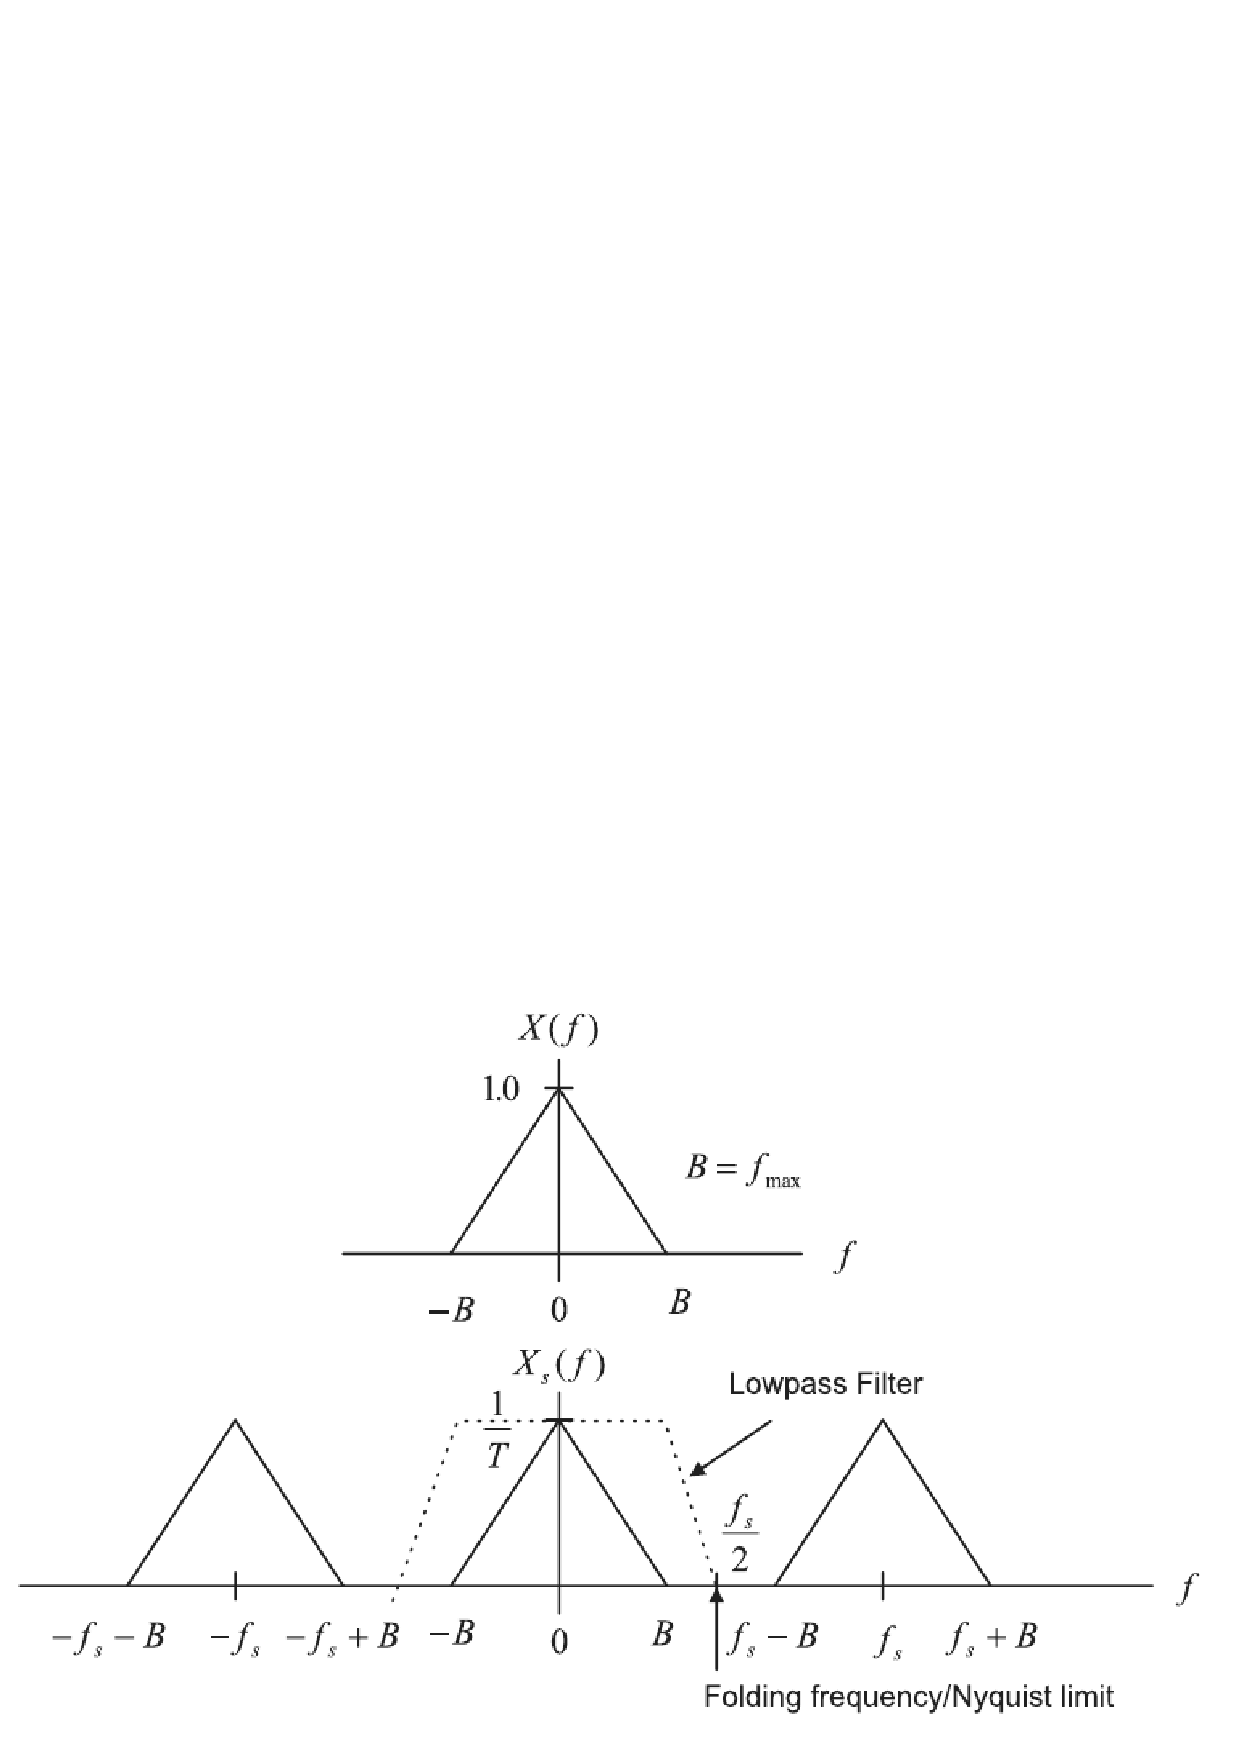
\includegraphics[width=0.5\linewidth]{./img/img09.png}
        \end{figure}
    \end{itemize}    
\end{frame}

\begin{frame}{Example}
    \begin{enumerate}[a.]
        \item Calculate the filter coefficients for a three-tap (number of coefficients) FIR lowpass filter with a cutoff frequency of 800 Hz and a sampling rate of 8000 Hz using the Fourier transform method.
        \item Determine the transfer function and difference equation of the designed FIR system.
        \item Compute and plot the magnitude frequency response for $\Omega = 0$, $\pi/4$, $\pi/2$, $3\pi/4$, and $\pi$ (rad).
    \end{enumerate}
\end{frame}

\begin{frame}{Solution}
    \begin{enumerate}[a.]
        \item The normalized cutoff frequency:$$ \Omega_c = 2 \pi f_c/f_s = \frac{2 \pi \cdot 800 }{8000} = 0.2 \pi \text{ (rad)}$$
        3-tap FIR lowpass filter $\rightarrow$ 3 coefficients $\rightarrow$ $2M + 1 = 3$ $\rightarrow$ M = 1, filter coefficients:
        \begin{align*}
            h(0) &= \frac{\Omega_c}{\pi} = \frac{0.2 \pi}{\pi} = 0.2 \\
            h(1) &= \frac{\sin(\Omega_c n)}{n \pi} = \frac{\sin(0.2 \pi \cdot 1)}{1 \cdot \pi}  = 0.1871 \\
            h(-1) &= h(1) = 0.1871
        \end{align*}
    \end{enumerate}
\end{frame}

\begin{frame}{Solution}
    \begin{enumerate}[a.]
        \setcounter{enumi}{1}
        \item[] delaying $h(n)$ by $M=1$, then
        \begin{align*}
            b(0) &= h(0-1) = h(-1) = 0.1871 \\
            b(1) &= h(1-1) = h(0) = 0.2 \\
            b(2) &= h(2-1) = h(1) = 0.1871
        \end{align*}
        \item transfer function of the designed FIR system: $$ H(z) = 0.1871 + 0.2z^{-1} + 0.1871z^{-2} $$  difference equation of the designed FIR system: $$ y(n) = 0.1871x(n) + 0.2x(n-1) + 0.1871x(n-2) $$
    \end{enumerate}
\end{frame}

\begin{frame}{Solution}
    \begin{enumerate}[a.]
        \setcounter{enumi}{2}
        \item substitute $z = e^{j\Omega}$ $$ H(e^{j\Omega}) = 0.1871 + 0.2e^{-j\Omega} + 0.1871e^{-j2\Omega} $$ factoring $e^{-j\Omega}$ and using Euler formula $ e^{jx} + e^{-jx} = 2 \cos(x) $:
        \begin{align*}
            H(e^{j\Omega}) &= e^{-j\Omega}(0.1871e^{j\Omega} + 0.2 + 0.1871e^{-j\Omega}) \\
            &= e^{-j\Omega} (0.2 + 0.3742\cos(\Omega)) \\
            &= (0.2 + 0.3742\cos(\Omega)) e^{-j\Omega}
        \end{align*} magnitude frequency response: $$|H(e^{j\Omega})| = |0.2 + 0.3742\cos(\Omega)|$$ 
    \end{enumerate}
\end{frame}

\begin{frame}{Solution}
    \begin{enumerate}[a.]
        \item[] phase response: $$ \angle H(e^{j\Omega}) = \begin{cases}
            -\Omega & \text{ if } 0.2 + 0.3472\cos \Omega > 0 \\
            -\Omega + \pi & \text{ if } 0.2 + 0.3472\cos \Omega < 0
        \end{cases}$$
    \end{enumerate}
    \begin{figure}
        \centering
        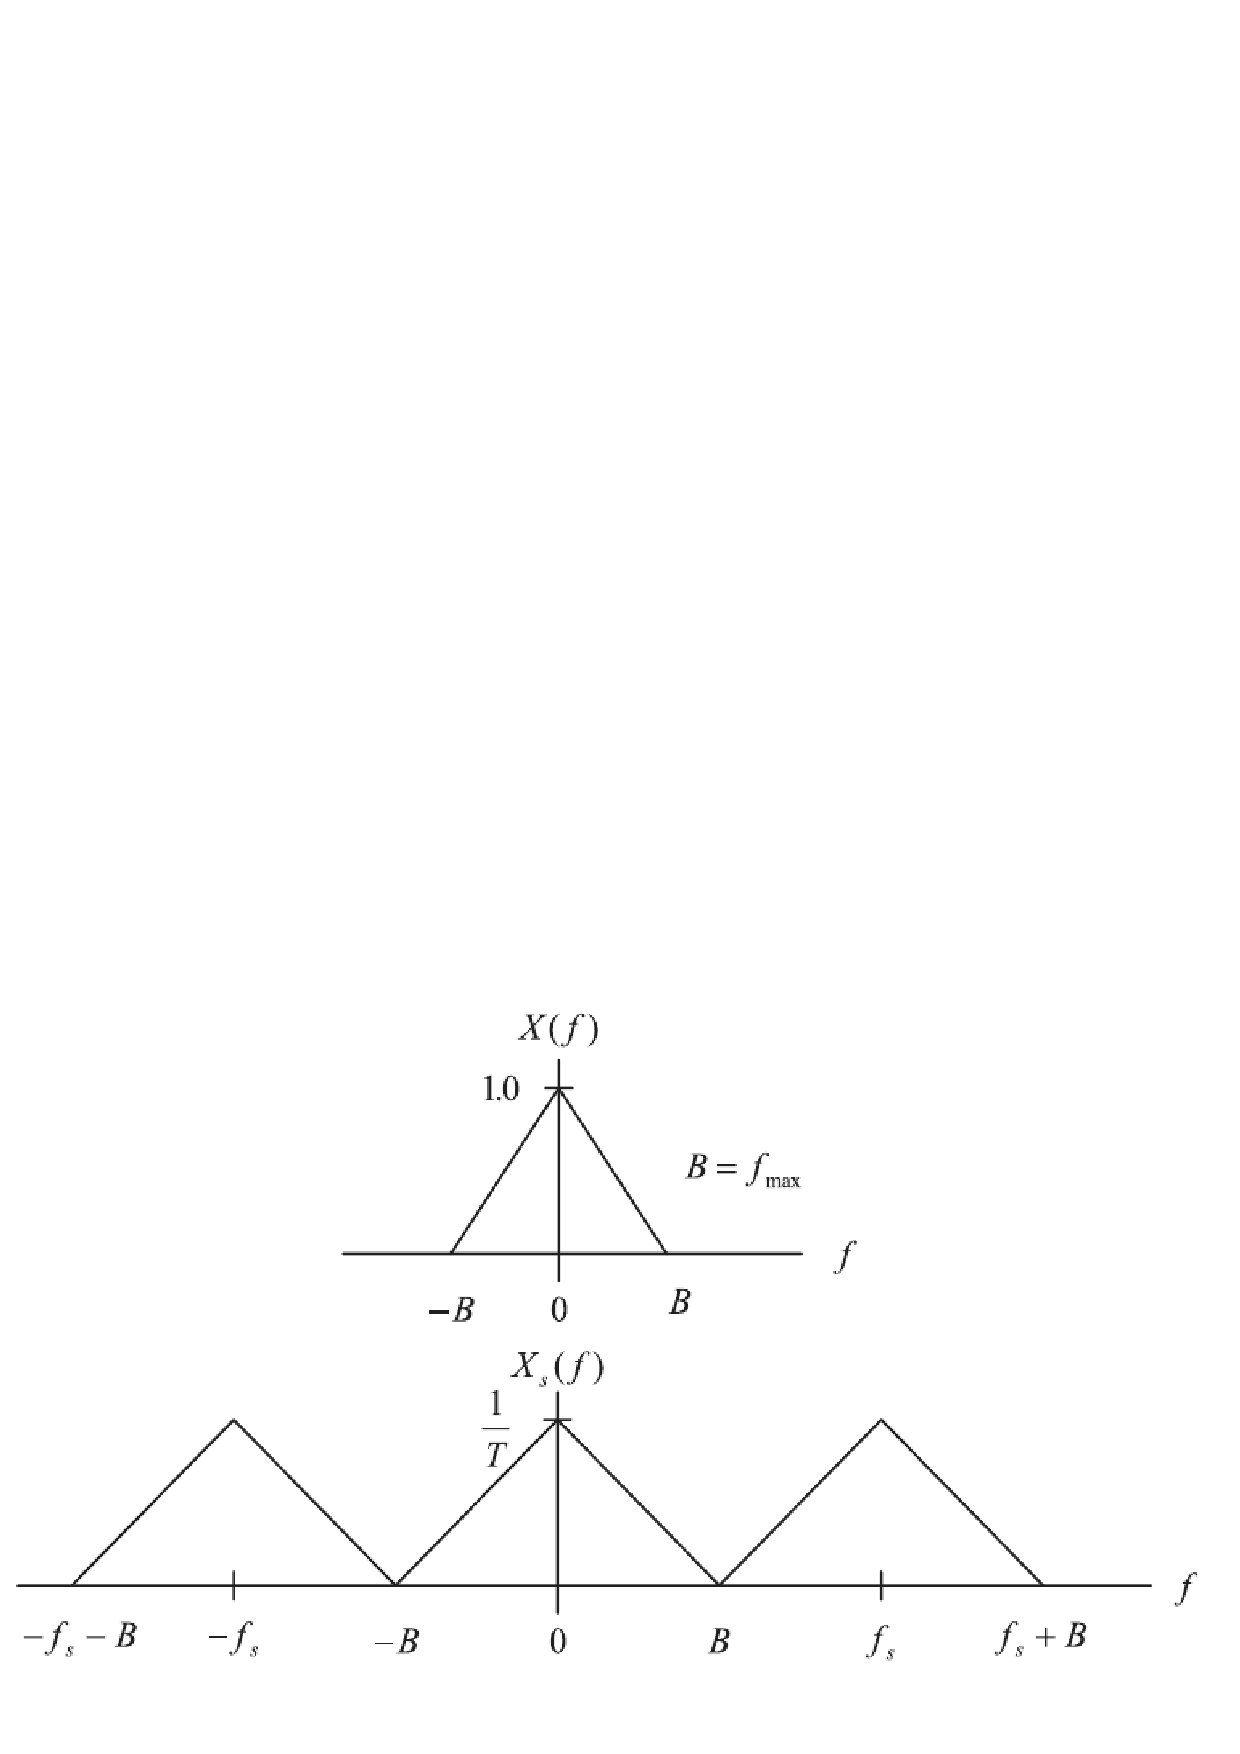
\includegraphics[width=\linewidth]{./img/img10.png}
    \end{figure}
\end{frame}

\begin{frame}{Solution}
    \begin{figure}
        \centering
        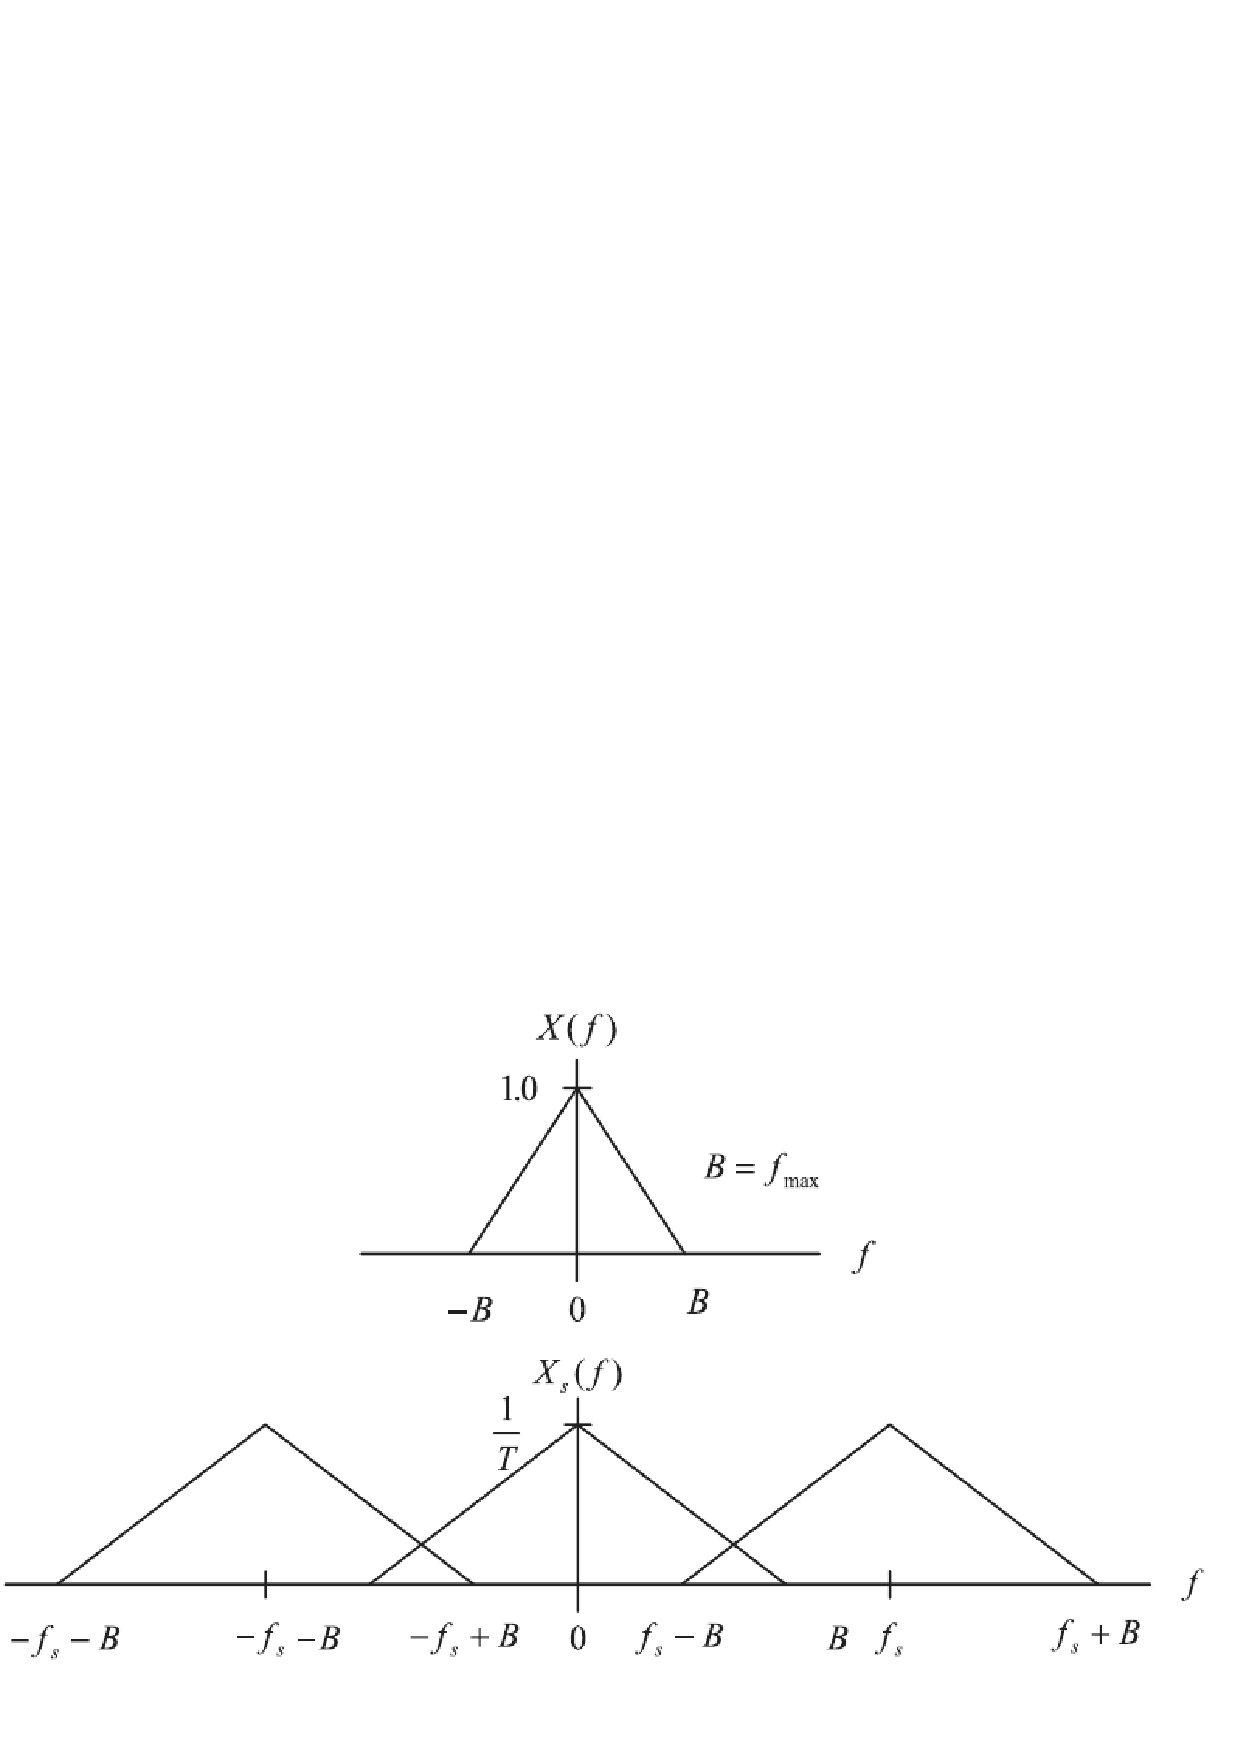
\includegraphics[width=0.8\linewidth]{./img/img11.png}
    \end{figure}
\end{frame}

\begin{frame}[fragile]{Python Code}
    \begin{minted}[frame=lines,framesep=2mm,fontsize=\tiny,bgcolor=LightGray]{python}
from scipy import signal
import matplotlib.pylab as plt
import numpy as np

fs = 8000
b = np.array([0.1871, 0.2, 0.1871])
w, h = signal.freqz(b)
plt.figure(figsize=(10,3))
plt.title('Digital filter frequency response')
plt.plot(w*fs/(2*np.pi), 20 * np.log10(abs(h)), 'b')
plt.ylabel('Magnitude (dB)', color='b')
plt.xlabel('Frequency (Hz)')
plt.legend(['3-tap FIR'], loc='lower left')
plt.grid()
plt.show()
    \end{minted}
\end{frame}

\begin{frame}{Result from Python Code}
    \begin{figure}
        \centering
        \includegraphics[width=\linewidth]{./img/img11a.png}
    \end{figure}
\end{frame}

\begin{frame}[fragile]{Python Code}
    \begin{minted}[frame=lines,framesep=2mm,fontsize=\tiny,bgcolor=LightGray]{python}
from scipy import signal
import matplotlib.pylab as plt
import numpy as np

fs = 8000
b = np.array([0.1871, 0.2, 0.1871])
w, h = signal.freqz(b)
angles = np.unwrap(np.angle(h))
plt.figure(figsize=(10,3))
plt.title('Digital filter frequency response')
plt.plot(w*fs/(2*np.pi), angles*180/np.pi, 'g')
plt.ylabel('Phase (Degree)', color='g')
plt.xlabel('Frequency (Hz)')
plt.legend(['3-tap FIR'], loc='lower left')
plt.grid()
plt.show()
    \end{minted}
\end{frame}

\begin{frame}{Result from Python Code}
    \begin{figure}
        \centering
        \includegraphics[width=\linewidth]{./img/img11b.png}
    \end{figure}
\end{frame}

\begin{frame}{Example}
    \begin{enumerate}[a.]
        \item Calculate the filter coefficients for a \textbf{17-tap} (number of coefficients) FIR lowpass filter with a cutoff frequency of 800 Hz and a sampling rate of 8000 Hz using the Fourier transform method.
        \item Compute and plot the magnitude frequency response for $\Omega = 0$, $\pi/4$, $\pi/2$, $3\pi/4$, and $\pi$ (rad).
    \end{enumerate}
\end{frame}

\begin{frame}{Solution}
    \begin{enumerate}[a.]
        \item 17-tap (number of coefficients) $\rightarrow$ M = 8
    \end{enumerate}
    \begin{figure}
        \centering
        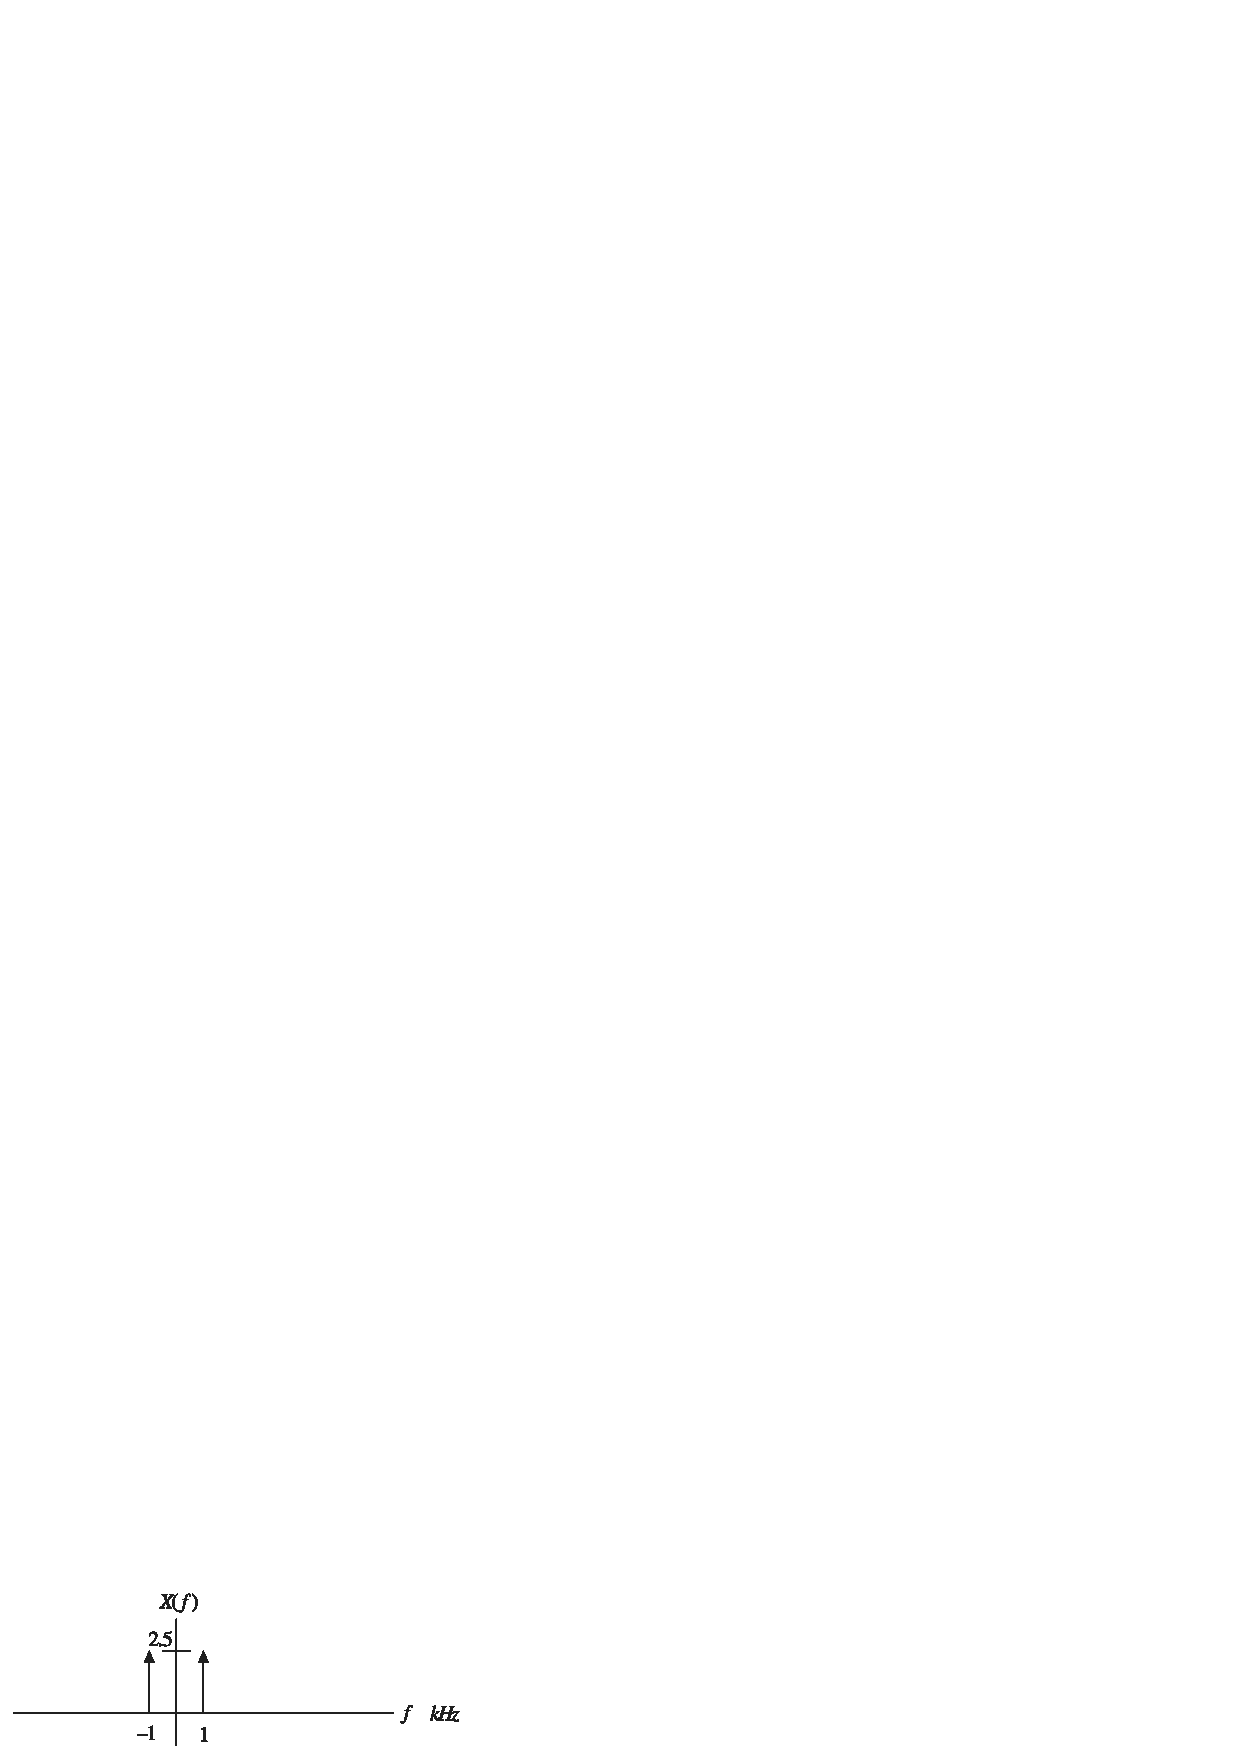
\includegraphics[width=\linewidth]{./img/img12.png}
    \end{figure}
\end{frame}

\begin{frame}{Solution}
    \begin{enumerate}[a.]
        \setcounter{enumi}{1}
        \item magnitude freq and phase resp.
    \end{enumerate}
    \begin{figure}
        \centering
        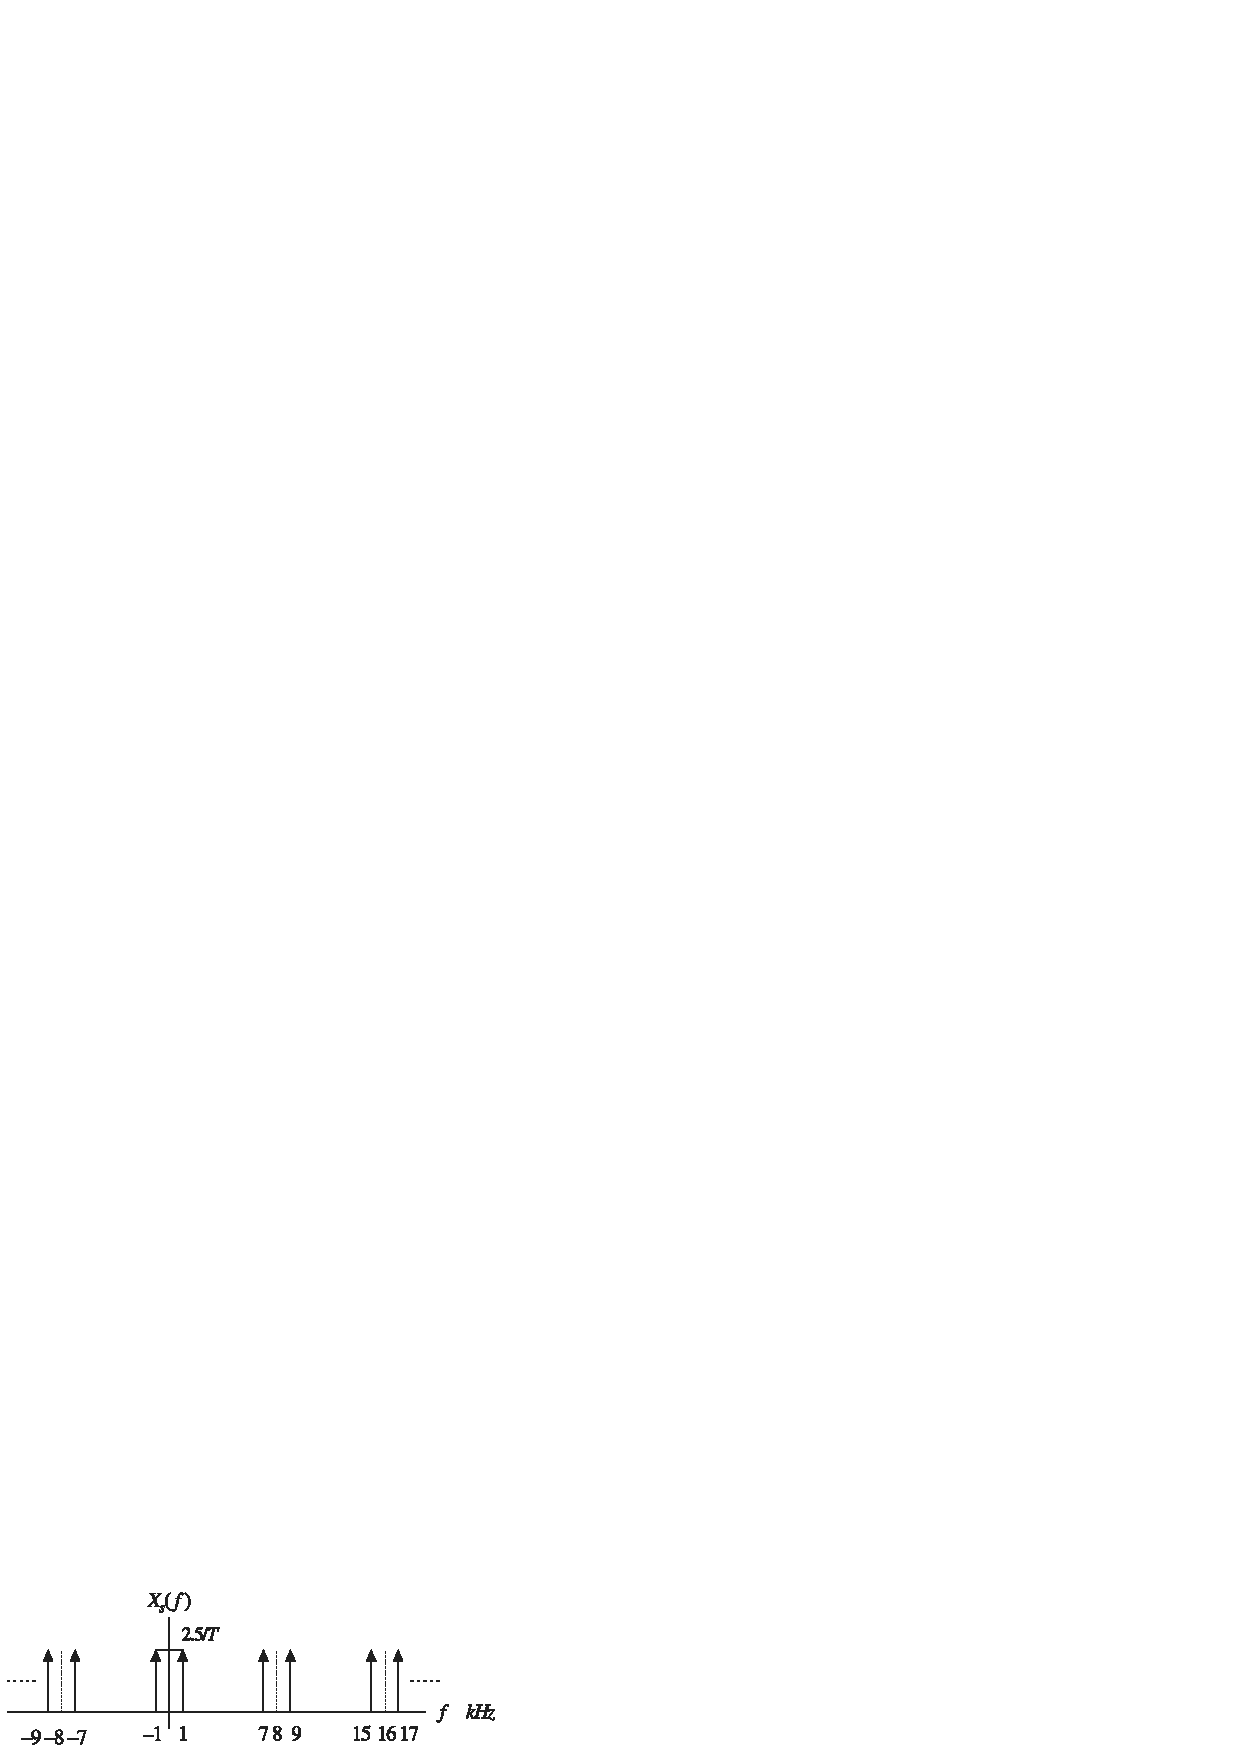
\includegraphics[width=0.7\linewidth]{./img/img13.png}
    \end{figure}
\end{frame}

\begin{frame}[fragile]{Python Code}
    \begin{minted}[frame=lines,framesep=2mm,fontsize=\tiny,bgcolor=LightGray]{python}
from scipy import signal
import matplotlib.pylab as plt
import numpy as np

fs = 8000
b = np.array([-0.0378, -0.0432, -0.0312, 0, 0.0468, 0.1009, 0.1514, 
                0.1871, 0.2, 0.1871, 0.1514, 0.1009, 0.0468, 0, -0.0312, -0.0432, -0.0378])
w, h = signal.freqz(b)
plt.figure(figsize=(10,3))
plt.title('Digital filter frequency response')
plt.plot(w*fs/(2*np.pi), 20 * np.log10(abs(h)), 'b')
plt.ylabel('Magnitude (dB)', color='b')
plt.xlabel('Frequency (Hz)')
plt.legend(['17-tap FIR'], loc='lower left')
plt.grid()
plt.show()
    \end{minted}
\end{frame}

\begin{frame}{Result from Python Code}
    \begin{figure}
        \centering
        \includegraphics[width=\linewidth]{./img/img14.png}
    \end{figure}
\end{frame}

\begin{frame}[fragile]{Python Code}
    \begin{minted}[frame=lines,framesep=2mm,fontsize=\tiny,bgcolor=LightGray]{python}
from scipy import signal
import matplotlib.pylab as plt
import numpy as np

fs = 8000
b = np.array([-0.0378, -0.0432, -0.0312, 0, 0.0468, 0.1009, 0.1514, 
                0.1871, 0.2, 0.1871, 0.1514, 0.1009, 0.0468, 0, -0.0312, -0.0432, -0.0378])
w, h = signal.freqz(b)
angles = np.unwrap(np.angle(h))
plt.figure(figsize=(10,3))
plt.title('Digital filter frequency response')
plt.plot(w*fs/(2*np.pi), angles*180/np.pi, 'g')
plt.ylabel('Phase (Degree)', color='g')
plt.xlabel('Frequency (Hz)')
plt.legend(['17-tap FIR'], loc='lower left')
plt.grid()
plt.show()
plt.show()
    \end{minted}
\end{frame}

\begin{frame}{Result from Python Code}
    \begin{figure}
        \centering
        \includegraphics[width=\linewidth]{./img/img15.png}
    \end{figure}
\end{frame}

\begin{frame}{Compare 3-tap and 17-tap FIR filter}
    \begin{figure}
        \centering
        \includegraphics[width=\linewidth]{./img/img16.png}
        \includegraphics[width=\linewidth]{./img/img17.png}
    \end{figure}
\end{frame}

\begin{frame}{FIR Filter frequency response}
    \begin{itemize}
        \item Ripples $\rightarrow$ \textbf{Gibbs effect}
        \item To remedy this problem, \textbf{window functions} will be used
        \item larger number of the filter coefficients:
        \begin{itemize}
            \item produce the sharp roll-off characteristic of the transition band
            \item but may cause increased time delay and increase computational complexity for implementing the designed FIR filter
        \end{itemize}
    \end{itemize}
\end{frame}

\begin{frame}{FIR Filter Coefficients:\\Window method}
    \begin{itemize}
        \item Applying the window sequence to the filter coefficients gives $$ h_w(n) = h(n) \cdot w(n) $$ where $w(n)$ designates the window function
        \item Common window functions:
        \begin{enumerate}[a.]
            \item Rectangular window:
            \begin{figure}
                \centering
                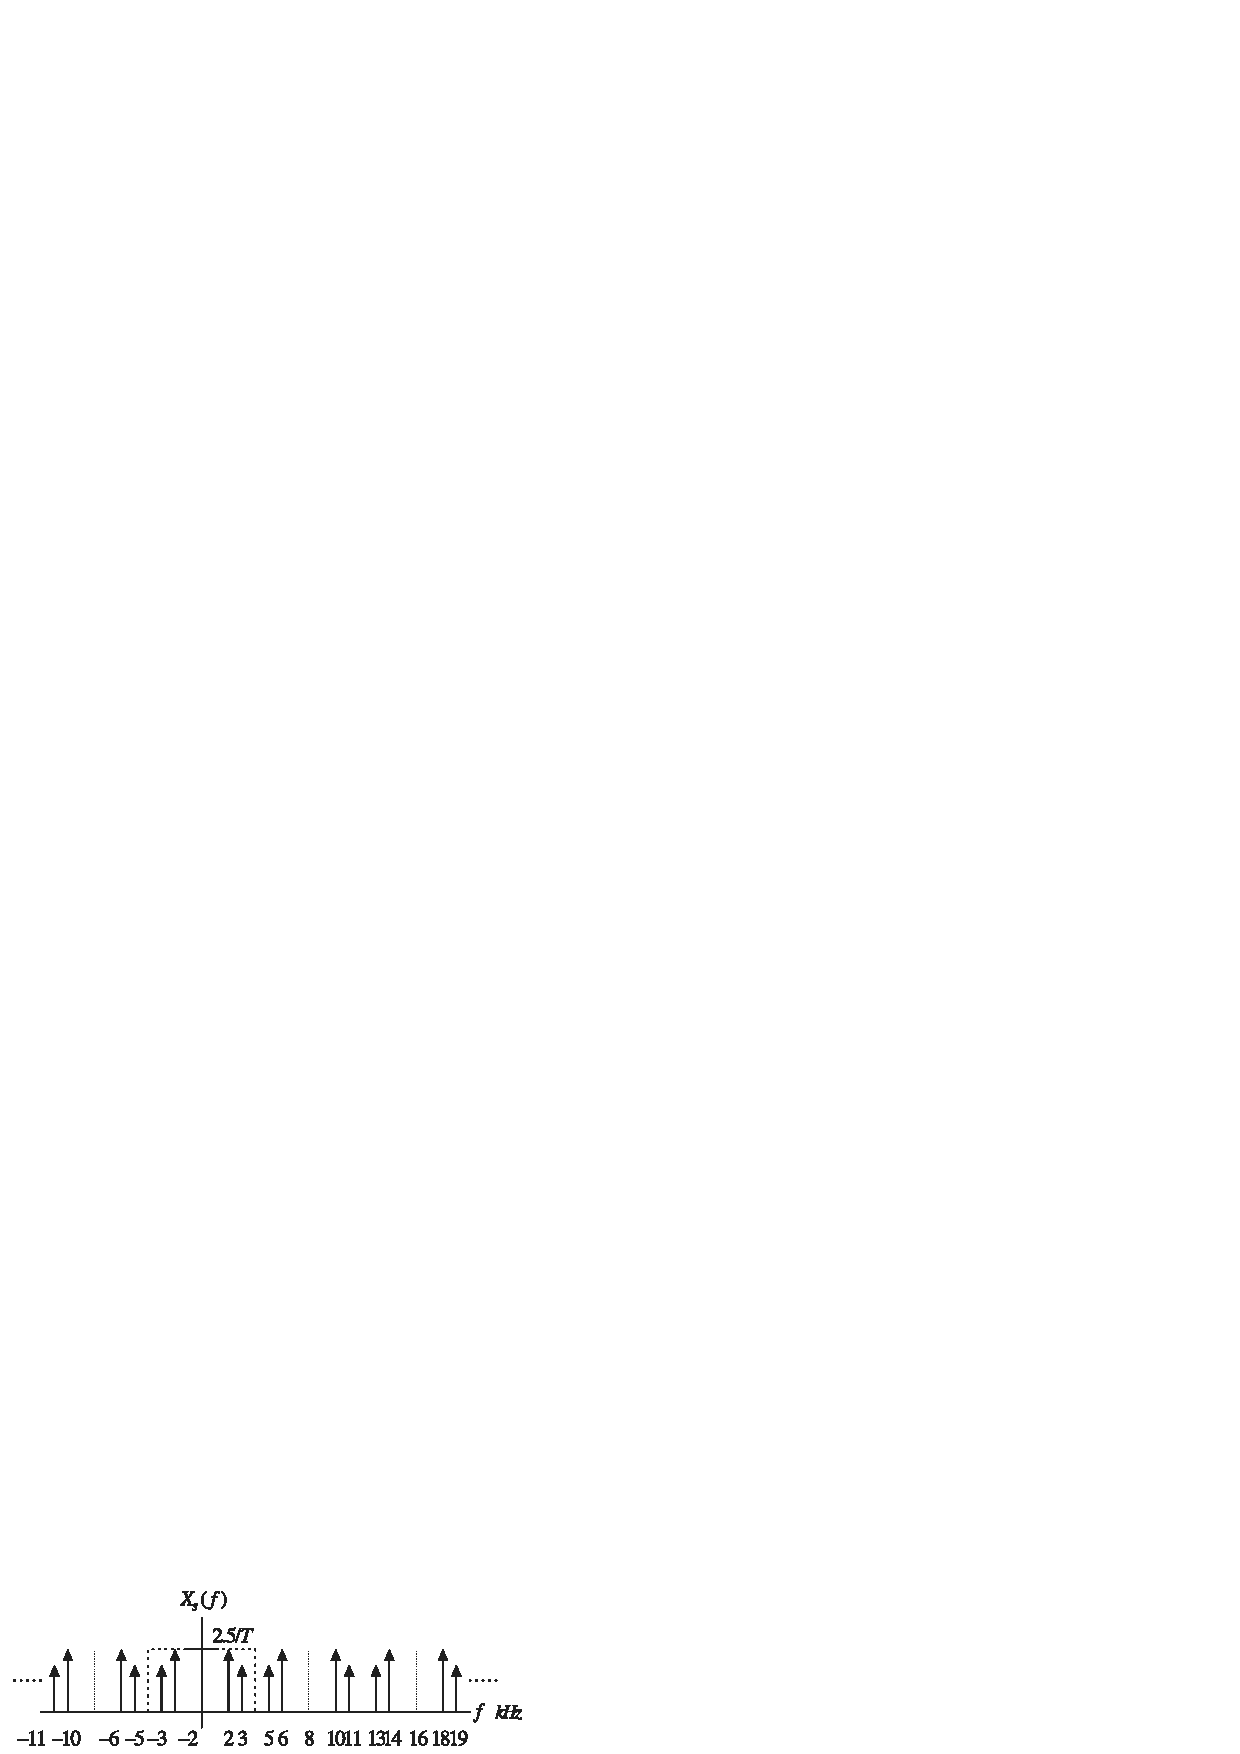
\includegraphics[width=0.5\linewidth]{./img/img18.png}
            \end{figure}
            \item Triangular(Bartlett) window:
            \begin{figure}
                \centering
                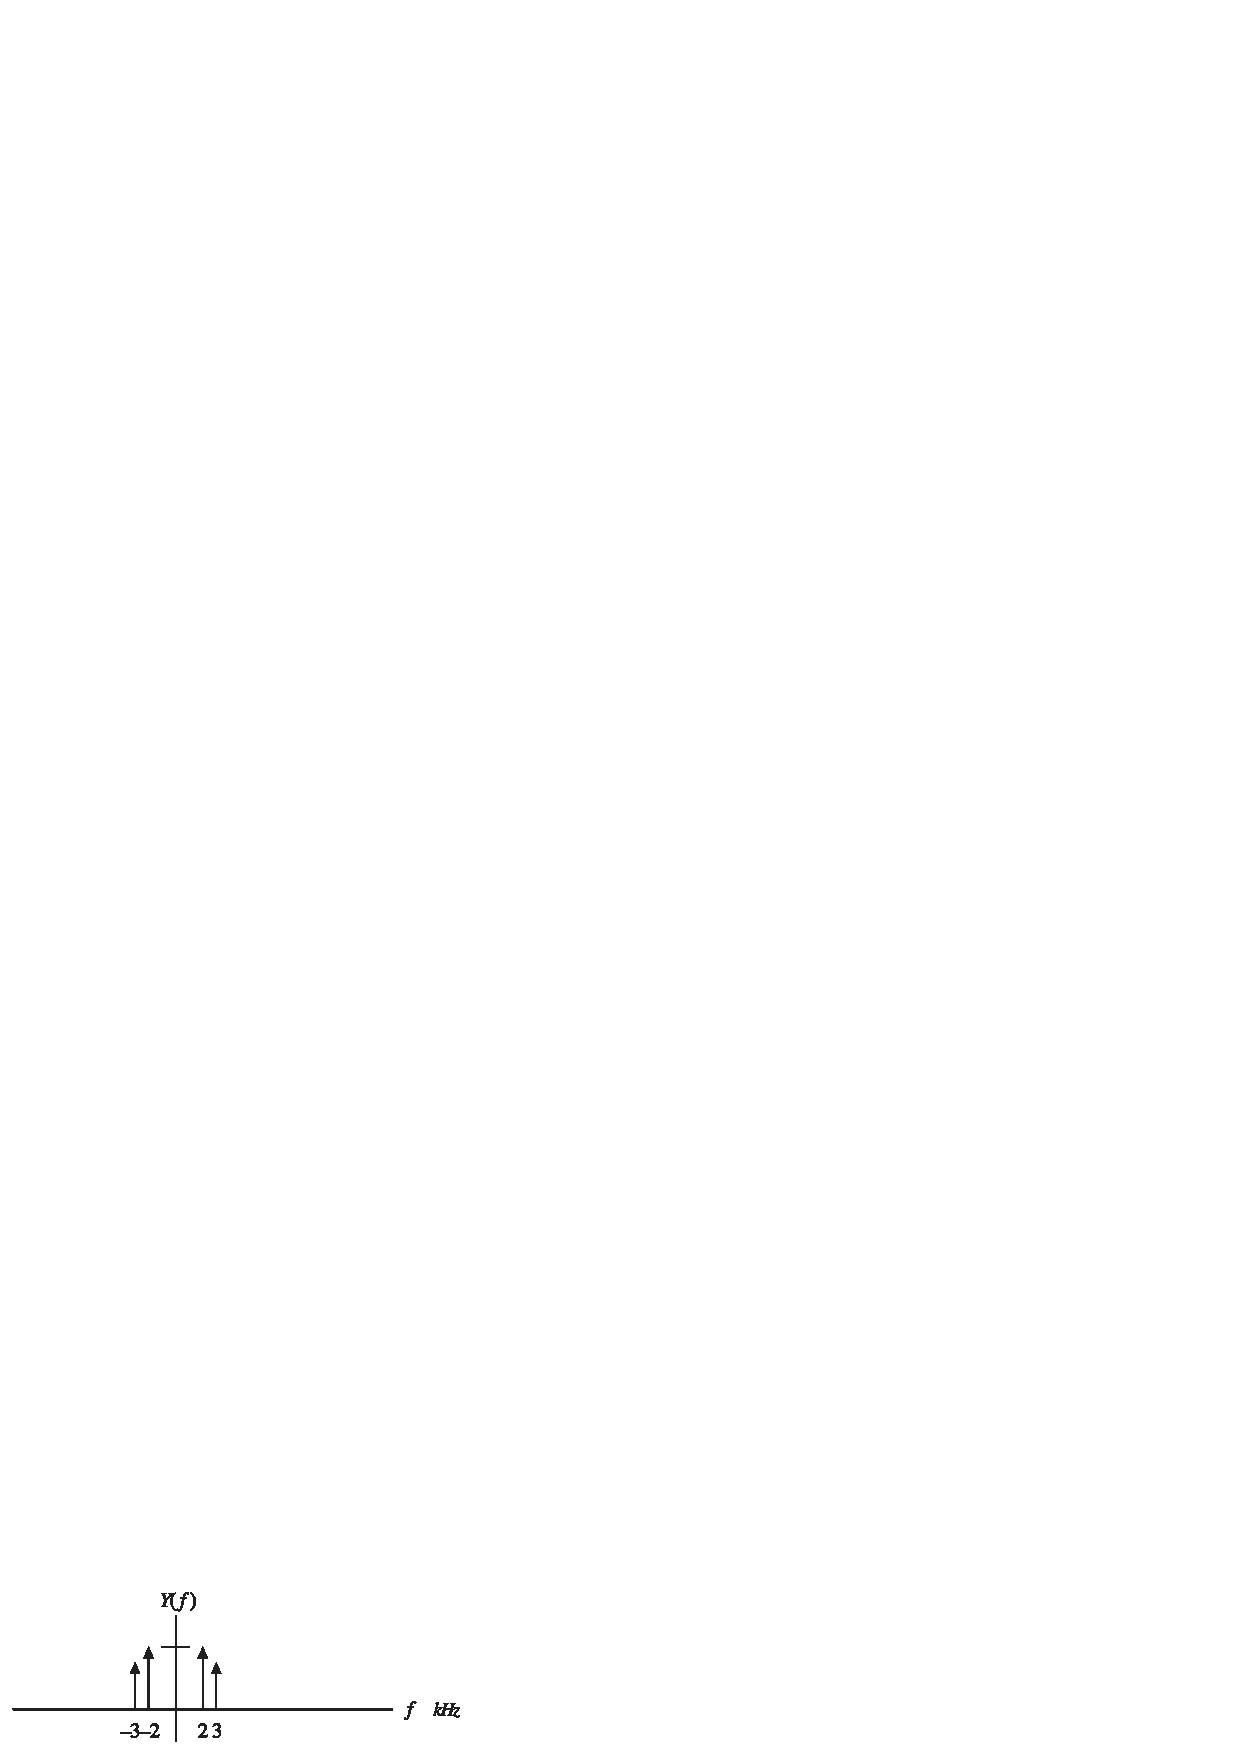
\includegraphics[width=0.5\linewidth]{./img/img19.png}
            \end{figure}
        \end{enumerate}
    \end{itemize}
\end{frame}

\begin{frame}{FIR Filter Coefficients:\\Window method}
    \begin{itemize}
        \item[]
        \begin{enumerate}[a.]
            \setcounter{enumi}{2}
            \item Hanning window:
            \begin{figure}
                \centering
                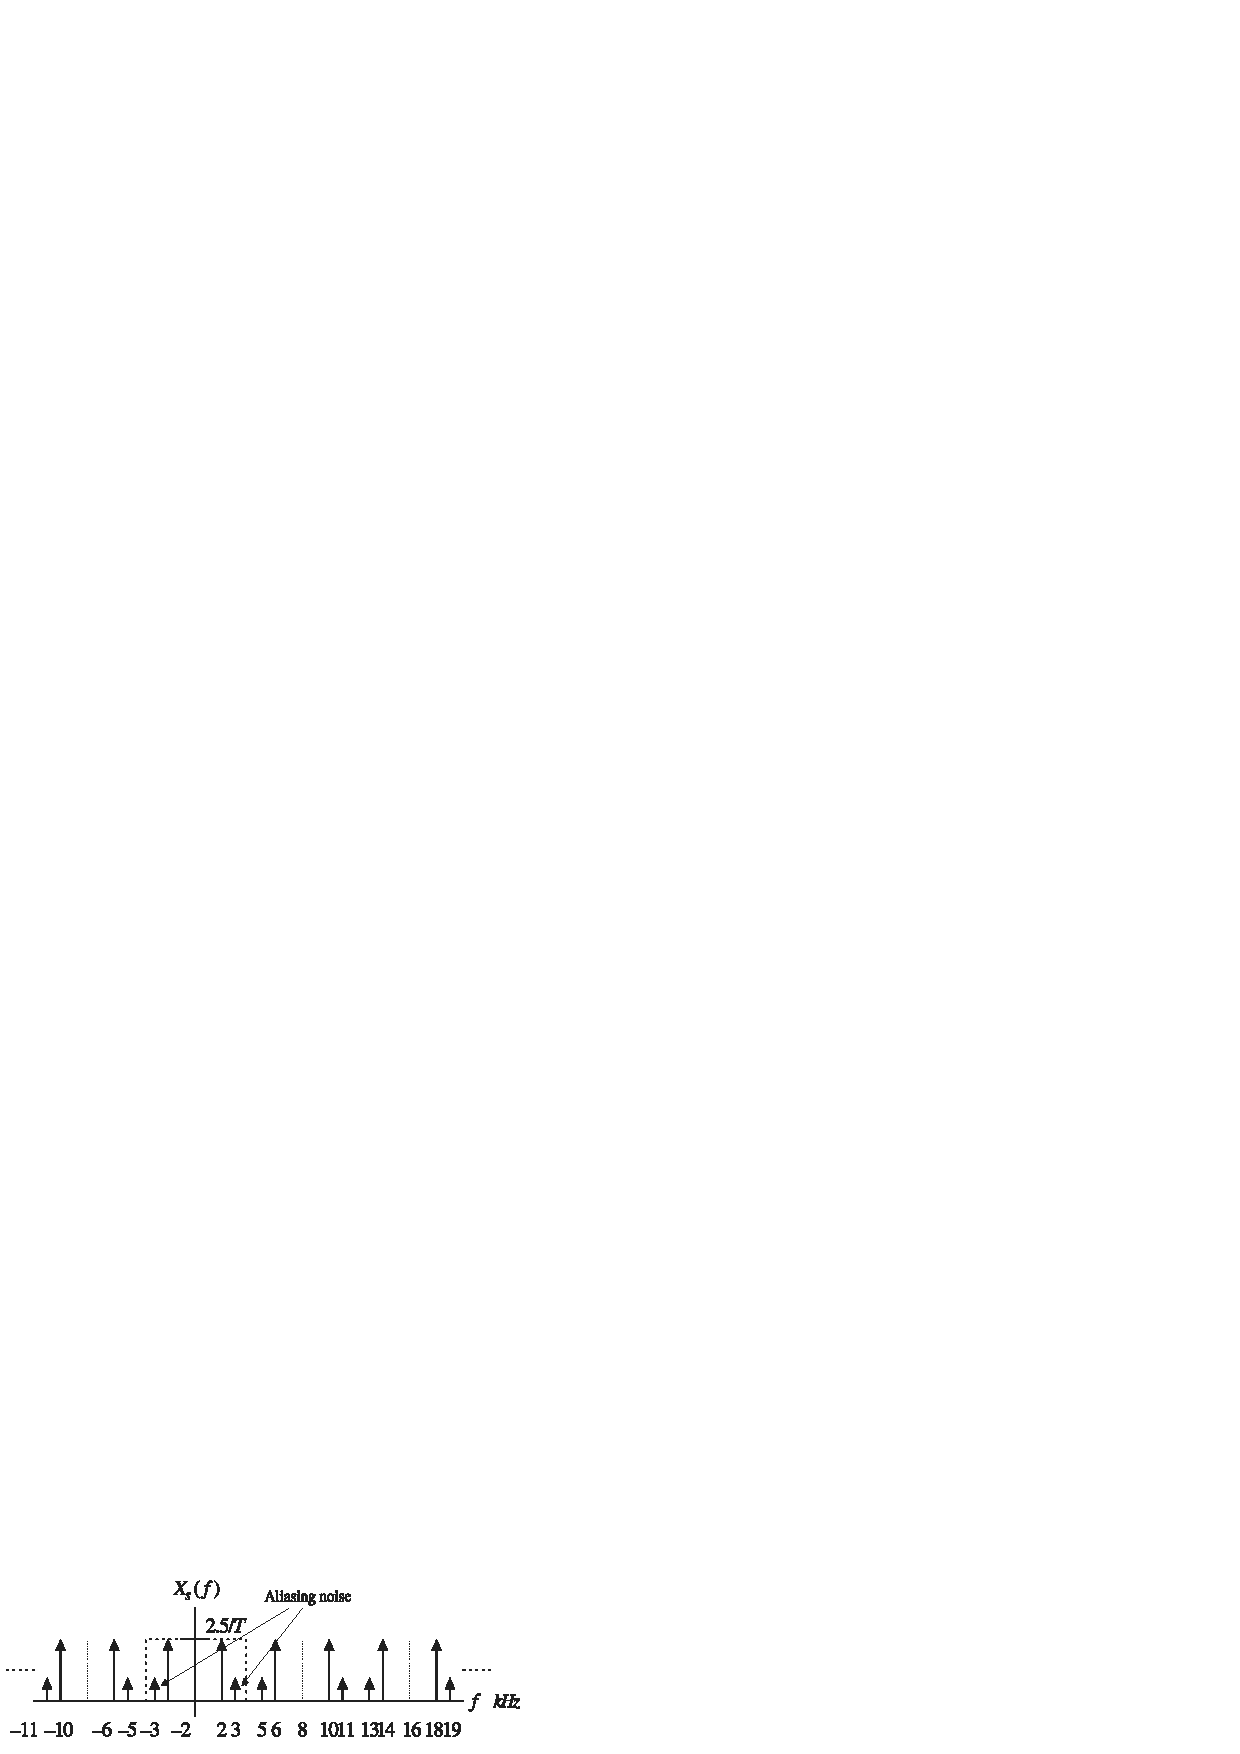
\includegraphics[width=0.7\linewidth]{./img/img20.png}
            \end{figure}
            \item Hamming window:
            \begin{figure}
                \centering
                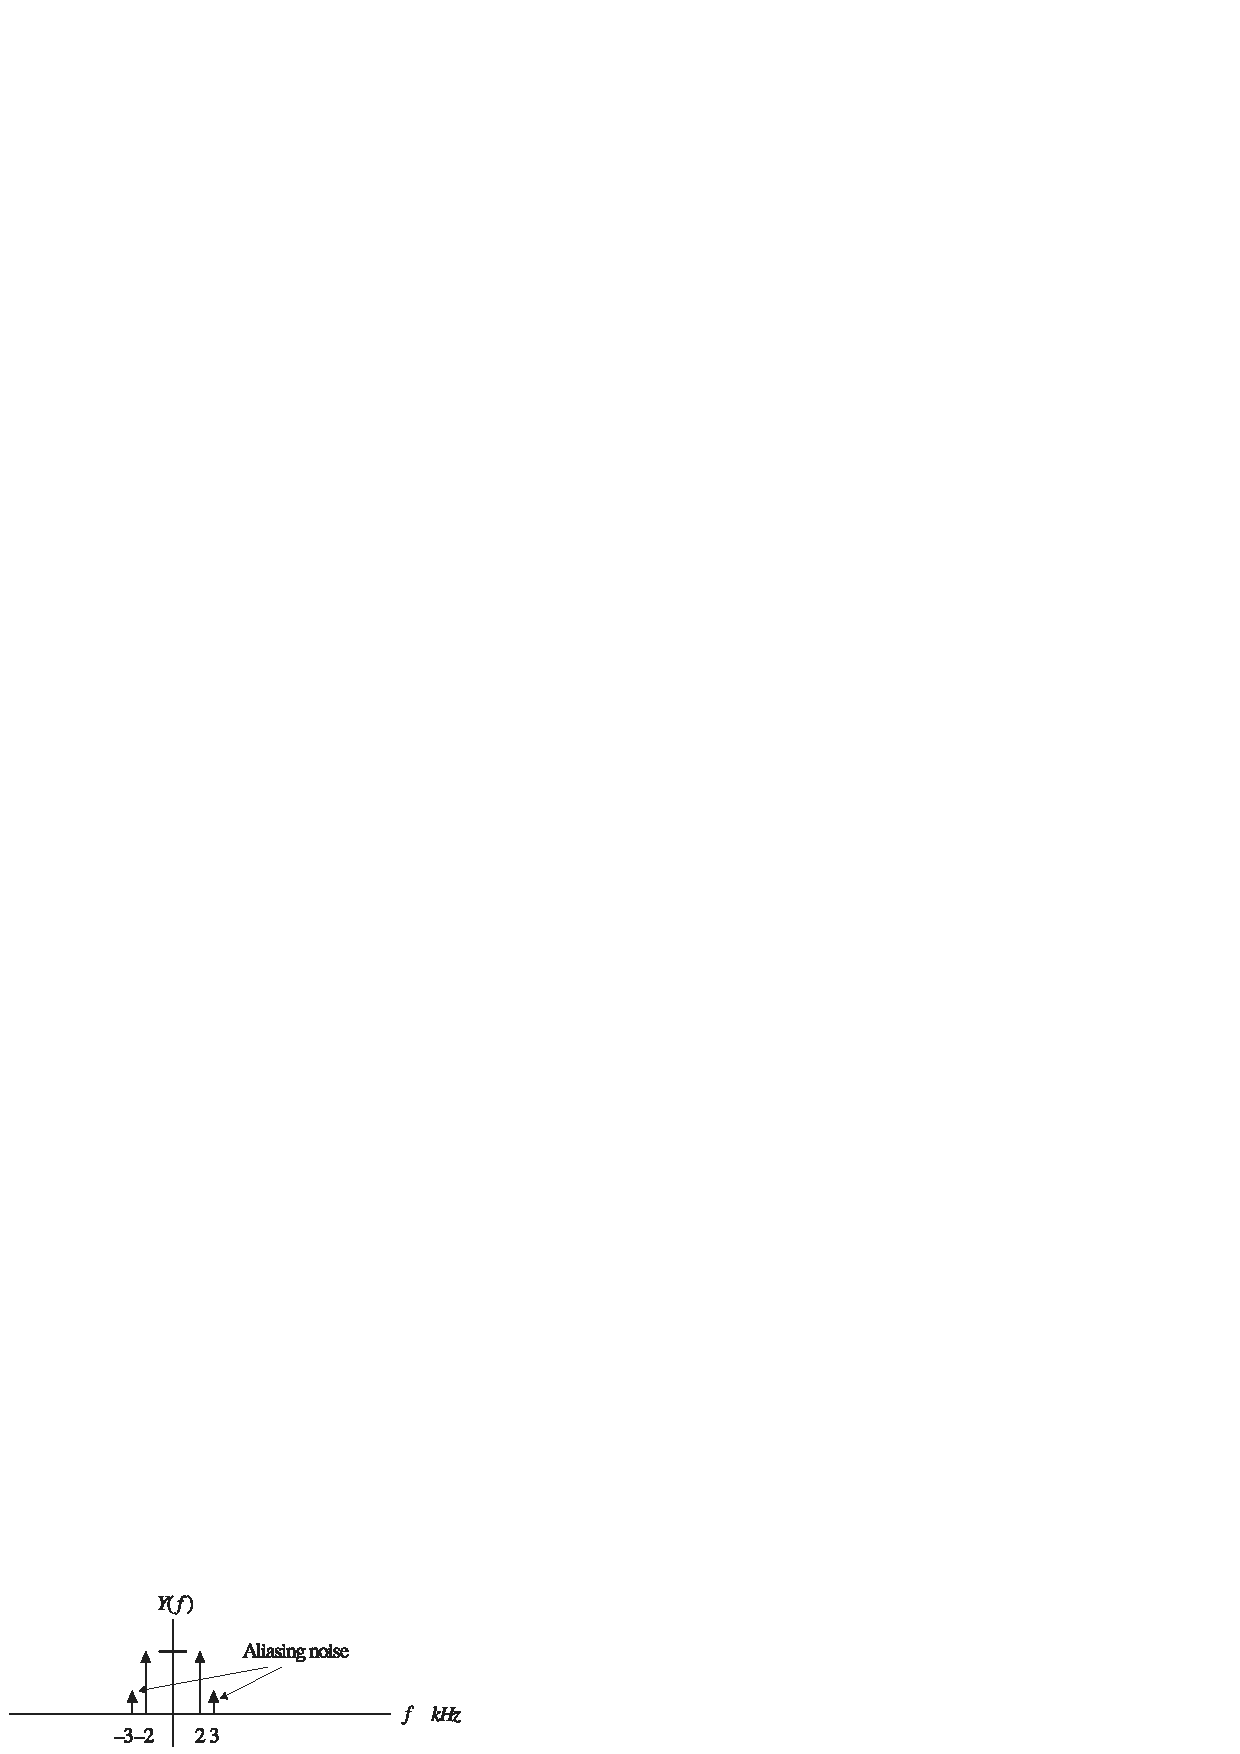
\includegraphics[width=0.7\linewidth]{./img/img21.png}
            \end{figure}
            \item Blackman window:
            \begin{figure}
                \centering
                \includegraphics[width=0.9\linewidth]{./img/img22.png}
            \end{figure}
        \end{enumerate}
    \end{itemize}
\end{frame}

\begin{frame}{Example}
    \begin{enumerate}[a.]
        \item Design a three-tap FIR lowpass filter with a cutoff frequency of 800 Hz and a sampling rate of 8000 Hz using the Hamming window function.
        \item Determine the transfer function and difference equation of the designed FIR system.
        \item Compute and plot the magnitude frequency response for $\Omega = 0$, $\pi/4$, $\pi/2$, $3\pi/4$, and $\pi$ (rad).
    \end{enumerate}
\end{frame}

\begin{frame}{Solution}
    \begin{enumerate}[a.]
        \item Cutoff frequency: $$\Omega_c = 2\pi f_c /f_s = 2 \pi \frac{800}{8000} = 0.2 \pi (rad)$$. $$2M+1 = 3 \rightarrow M = 1$$ FIR coef. $$h(n) = \frac{\Omega_c}{\pi} \rightarrow h(0) = \frac{0.2 \pi}{\pi} = 0.2$$ $$h(n) = \frac{\sin(\Omega_c n)}{n \pi} \rightarrow h(1) = \frac{\sin(0.2 \pi \cdot 1)}{1 \cdot \pi}= 0.1871 = h(-1)$$
    \end{enumerate}
\end{frame}

\begin{frame}{Solution}
    \begin{enumerate}[a.]
        \item[] Applying Hamming window:
        \begin{align*}
            w_{ham}(n) &= 0.54 + 0.46 \cos(\frac{n \pi}{1}) \\
            w_{ham}(0) &= 0.54 + 0.46 \cos(\frac{0 \cdot \pi}{1}) = 1 \\
            w_{ham}(1) &= 0.54 + 0.46 \cos(\frac{1 \cdot \pi}{1}) = 0.08 \\
            w_{ham}(-1) &= w_{ham}(1) = 0.08 \\
        \end{align*}
        windowed impulse response
        \begin{align*}
            h_w(0) &= h(0) \cdot w_{ham}(0) = 0.2 \cdot 1 = 0.2 \\
            h_w(1) &= h(1) \cdot w_{ham}(1) = 0.1871 \cdot 0.08 = 0.01497 \\
            h_w(-1) &= h(-1) \cdot w_{ham}(-1) = h(1) \cdot w_{ham}(1) = 0.01497 \\
        \end{align*}
    \end{enumerate}
\end{frame}

\begin{frame}{Solution}
    \begin{enumerate}[a.]
        \setcounter{enumi}{1}
        \item[] delaying $h_w(n)$ by $M = 1$
        $$ b_0 = b_2 = 0.01496 $$
        $$ b_1= 0.2 $$
        \item transfer function:
        $$ H(z) = 0.01497 + 0.2 z^{-1} + 0.01497z^{-2}$$
        $$ Y(z) = 0.01497X(z) + 0.2 z^{-1} X(z) + 0.01497z^{-2} X(z)$$
        $$ y(n) = 0.01497x(n) + 0.2 x(n-1) + 0.01497 x(n-2)$$
    \end{enumerate}
\end{frame}

\begin{frame}{Solution}
    \begin{enumerate}[a.]
        \setcounter{enumi}{2}
        \item  magnitude frequency response and phase response:
        \begin{align*}
            H(e^{j \Omega}) &= 0.01497 + 0.2 e^{-j \Omega} + 0.01497e^{-j2 \Omega} \\
            &= e^{-j \Omega} (0.01497e^{j \Omega} + 0.2  + 0.01497e^{-j \Omega}) \\
            &= e^{-j \Omega} (0.2 + 0.02994 \cos \Omega) \\
            |H(e^{j \Omega})| &= |0.2 + 0.02994 \cos \Omega| \\ 
            \angle H(e^{j \Omega}) &= \begin{cases}
                - \Omega &\text{ if } 0.2 + 0.02994 \cos \Omega > 0 \\
                - \Omega + \pi &\text{ if } 0.2 + 0.02994 \cos \Omega < 0
            \end{cases}
        \end{align*}
    \end{enumerate}
\end{frame}

\begin{frame}{Solution}
    \begin{figure}
        \centering
        \includegraphics[width=\linewidth]{./img/img23.png}
    \end{figure}
\end{frame}

\begin{frame}{Solution}
    \begin{figure}
        \centering
        \includegraphics[width=\linewidth]{./img/img24.png}
    \end{figure}
\end{frame}

\begin{frame}{Solution}
    \begin{figure}
        \centering
        \includegraphics[width=\linewidth]{./img/img25.png}
    \end{figure}
\end{frame}

\begin{frame}{Realization: Transversal Form}
    \begin{itemize}
        \item Example: Given an FIR filter transfer function $$ H(z) = 1 + 1.2z^{-1} + 0.36z^{-2} $$ perform the FIR filter realization.
        \item Solution: Obtain $b_0 = 1$, $b_1 = 1.2$, and $b_2 = 0.36$ $$ y(n) = x(n) + 1.2x(n-1) + 0.36x(n-2) $$
    \end{itemize}
\end{frame}

\begin{frame}{Realization: Transversal Form}
    \begin{figure}
        \centering
        \includegraphics[width=0.8\linewidth]{./img/img26.png}
    \end{figure}
\end{frame}

\begin{frame}{Realization: Linear Phase Form}
    \begin{itemize}
        \item Transfer function:
        $$ H(z) = b_0 + b_1z^{-1} + b_2z^{-2} + b_1z^{-3} + b_0z^{-4} $$
        \item Diff. equation:
        $$ y(n) = b_0x(n) + b_1x(n-1) + b_2x(n-2) + b_1x(n-3) + b_0x(n-4) $$
        \item then:
        $$ y(n) = b_0(x(n) + x(n-4)) + b_1(x(n-1) + x(n-3)) + b_2x(n-2) $$
    \end{itemize}
\end{frame}

\begin{frame}{Realization: Linear Phase Form}
    \begin{figure}
        \centering
        \includegraphics[width=0.8\linewidth]{./img/img27.png}
    \end{figure}
\end{frame}

\end{document}